% Working revision: journal-neutral source; PDF not rebuilt or visually verified.
% Options for packages loaded elsewhere
\PassOptionsToPackage{unicode}{hyperref}
\PassOptionsToPackage{hyphens}{url}
%
\documentclass[
]{article}
\usepackage{amsmath,amssymb}
\usepackage{iftex}
\ifPDFTeX
  \usepackage[T1]{fontenc}
  \usepackage[utf8]{inputenc}
  \usepackage{textcomp} % provide euro and other symbols
\else % if luatex or xetex
  \usepackage{unicode-math} % this also loads fontspec
  \defaultfontfeatures{Scale=MatchLowercase}
  \defaultfontfeatures[\rmfamily]{Ligatures=TeX,Scale=1}
\fi
\usepackage{lmodern}
\ifPDFTeX\else
  % xetex/luatex font selection
\fi
% Use upquote if available, for straight quotes in verbatim environments
\IfFileExists{upquote.sty}{\usepackage{upquote}}{}
\IfFileExists{microtype.sty}{% use microtype if available
  \usepackage[]{microtype}
  \UseMicrotypeSet[protrusion]{basicmath} % disable protrusion for tt fonts
}{}
\makeatletter
\@ifundefined{KOMAClassName}{% if non-KOMA class
  \IfFileExists{parskip.sty}{%
    \usepackage{parskip}
  }{% else
    \setlength{\parindent}{0pt}
    \setlength{\parskip}{6pt plus 2pt minus 1pt}}
}{% if KOMA class
  \KOMAoptions{parskip=half}}
\makeatother
\usepackage{xcolor}
\usepackage[margin=25mm]{geometry}
\usepackage{longtable,booktabs,array}
\usepackage{calc} % for calculating minipage widths
% Correct order of tables after \paragraph or \subparagraph
\usepackage{etoolbox}
\makeatletter
\patchcmd\longtable{\par}{\if@noskipsec\mbox{}\fi\par}{}{}
\makeatother
% Allow footnotes in longtable head/foot
\IfFileExists{footnotehyper.sty}{\usepackage{footnotehyper}}{\usepackage{footnote}}
\makesavenoteenv{longtable}
\usepackage{graphicx}
\makeatletter
\def\maxwidth{\ifdim\Gin@nat@width>\linewidth\linewidth\else\Gin@nat@width\fi}
\def\maxheight{\ifdim\Gin@nat@height>\textheight\textheight\else\Gin@nat@height\fi}
\makeatother
% Scale images if necessary, so that they will not overflow the page
% margins by default, and it is still possible to overwrite the defaults
% using explicit options in \includegraphics[width, height, ...]{}
\setkeys{Gin}{width=\maxwidth,height=\maxheight,keepaspectratio}
% Set default figure placement to htbp
\makeatletter
\def\fps@figure{htbp}
\makeatother
\setlength{\emergencystretch}{3em} % prevent overfull lines
\providecommand{\tightlist}{%
  \setlength{\itemsep}{0pt}\setlength{\parskip}{0pt}}
\setcounter{secnumdepth}{-\maxdimen} % remove section numbering
\ifLuaTeX
  \usepackage{selnolig}  % disable illegal ligatures
\fi
\IfFileExists{bookmark.sty}{\usepackage{bookmark}}{\usepackage{hyperref}}
\IfFileExists{xurl.sty}{\usepackage{xurl}}{} % add URL line breaks if available
\urlstyle{same}
\hypersetup{
  hidelinks,
  pdfcreator={LaTeX via pandoc}}

\author{}
\date{}

\begin{document}

\hypertarget{supplementary-materials-for-a-decision-consequence-auditing-framework-for-reliable-surrogate-assisted-optimization-in-expensive-engineering-design}{%
\section{Supplementary Materials for A Decision-Consequence Auditing Framework for Reliable Surrogate-Assisted Optimization in Expensive Engineering Design}\label{supplementary-materials-for-a-decision-consequence-auditing-framework-for-reliable-surrogate-assisted-optimization-in-expensive-engineering-design}}

\textbf{Shu-Chuan Chu, Ya-Yu Zhang, Zhenyu Meng and Jia Zhao}

This document preserves secondary analyses, complete denominators, resource measurements, application transfer, high-dimensional extensions, sensitivity studies, and recovery accounting supporting the main article. The main article contains the prespecified primary BBOB contrasts and finite-element engineering results. No supplementary analysis reverses the failed development optimization-benefit gate.

\hypertarget{s0-evidence-map-and-reproducibility-checklist}{%
\section{S0 Evidence Map and Reproducibility Checklist}\label{s0-evidence-map-and-reproducibility-checklist}}

The supplement is organized by the claims made in the main article. Scientific results, resource measurements, and recovery records are separated so that interrupted physical calls and implementation checks cannot be mistaken for optimization evidence.

\hypertarget{s0.1-evidence-map}{%
\subsection{S0.1 Evidence map}\label{s0.1-evidence-map}}

\begin{enumerate}
\def\labelenumi{\arabic{enumi}.}
\tightlist
\item
  \textbf{Calibration and decision utility:} S1-S2, Tables S1-S7, and Figures S1-S4 provide declaration counts, failure fractions, common-history diagnostics, and common-state utility.
\item
  \textbf{External descriptive context:} S3, Tables S8-S12, and Figures S5-S6 report full BBOB endpoints and exclusive process costs under distinct search histories.
\item
  \textbf{Transfer evidence:} S4-S5, Tables S13-S19, and Figures S7-S10 cover LassoBench and the 300-dimensional experiment.
\item
  \textbf{Sensitivity:} S6-S7, Tables S20-S24, and Figures S11-S13 report model, training-cap, and total-budget sensitivity.
\item
  \textbf{Information order and accounting:} S7.3-S8.3 and Table S25 preserve finite-element replay, source hashes, recovery ledgers, and matched-initialization evidence.
\end{enumerate}

\hypertarget{s0.2-reproducibility-checklist}{%
\subsection{S0.2 Reproducibility checklist}\label{s0.2-reproducibility-checklist}}

\begin{enumerate}
\def\labelenumi{\arabic{enumi}.}
\tightlist
\item
  \textbf{Runtime:} Windows 11, Python 3.12.13, and dependency lock files for the main, application, GP, and reporting environments.
\item
  \textbf{Hardware:} AMD Ryzen 7 9700X, 16 logical threads, and approximately 31.1 GiB physical memory; numerical-library threads are limited to one per worker.
\item
  \textbf{Randomness:} Purpose-specific seed maps cover initialization, candidate generation, mode selection, optimization repeats, and bootstrap analyses.
\item
  \textbf{Protocols and parameters:} Frozen JSON configurations retain budgets, function and instance lists, model settings, and entry-point arguments.
\item
  \textbf{Information order:} PRE/LABEL journals, prediction-time training indices, candidate arrays, and separate diagnostic-label archives are retained.
\item
  \textbf{Integrity:} Source fingerprints, dependency hashes, raw-file hashes, endpoint replay, and expected aggregate tables are archived.
\item
  \textbf{Data and applications:} BBOB/COCO identifiers, fixed LassoBench datasets and splits, and the deterministic EngiBench finite-element parameterization are recorded.
\item
  \textbf{Recovery:} Incomplete units, canonical-versus-physical call ledgers, rerun seeds, and exclusion rules are archived separately.
\end{enumerate}

The manuscript sources, implementation, frozen configurations, and dependency records are available in the public repository https://github.com/ya-yu-zhang/Reliable-Surrogate-Assisted-Optimization-in-Expensive-Engineering-Design. Approximately 13.6 GB of raw experiment outputs and the full execution archives are not committed to that repository. The reported experiments can be regenerated using the documented environments and configurations; archived raw data are available from the corresponding author upon reasonable request. Public visibility should not be interpreted as an open-source license; third-party implementations and publisher templates retain their own terms. The detailed audit trail remains in S8; this map is a navigation layer rather than a substitute for those records.

\hypertarget{s1-development-diagnostics-and-common-state-evidence}{%
\section{S1 Development diagnostics and common-state evidence}\label{s1-development-diagnostics-and-common-state-evidence}}

\hypertarget{s1.1-exploration-failure-and-sparse-declarations}{%
\subsubsection{S1.1 Exploration, failure, and sparse declarations}\label{s1.1-exploration-failure-and-sparse-declarations}}

PEM-T explores approximately 36.6\% and 33.4\% of post-initialization evaluations, compared with approximately 10\% for the fixed control. Its observed failure fractions are approximately 9.9\% and 9.5\%. Being near the nominal monitoring level does not correspond to better endpoints.

\begin{longtable}[]{@{}lllllll@{}}
\caption{Joint closed-loop decision indicators, 72 runs per dimension/method}\tabularnewline
\toprule\noalign{}
D & Method & Exploration & Failure & Claims & False & Pooled FDP \\
\midrule\noalign{}
\endfirsthead
\toprule\noalign{}
D & Method & Exploration & Failure & Claims & False & Pooled FDP \\
\midrule\noalign{}
\endhead
\bottomrule\noalign{}
\endlastfoot
10 & PEM\_ST & 0.3574 & 0.1062 & 7 & 4 & 0.5714 \\
10 & PEM\_T & 0.3664 & 0.0986 & 3 & 1 & 0.3333 \\
10 & error\_only & 0.1574 & 0.0847 & 4 & 2 & 0.5000 \\
10 & fixed01 & 0.0995 & 0.0843 & 4 & 2 & 0.5000 \\
10 & stagnation\_only & 0.2338 & 0.0972 & 2 & 0 & 0.0000 \\
20 & PEM\_ST & 0.3478 & 0.1098 & 32 & 2 & 0.0625 \\
20 & PEM\_T & 0.3335 & 0.0946 & 0 & 0 & NA \\
20 & error\_only & 0.1475 & 0.0864 & 8 & 4 & 0.5000 \\
20 & fixed01 & 0.1017 & 0.0868 & 10 & 9 & 0.9000 \\
20 & stagnation\_only & 0.2394 & 0.0951 & 1 & 1 & 1.0000 \\
\end{longtable}

PEM-T makes only three declarations in dimension 10, one false, and no declarations in dimension 20. The latter FDP is NA, not zero. PEM-ST makes 32 declarations with two false in dimension 20, but its endpoint remains worse. Table S1's pooled declaration ratio is distinct from a mean over runs with nonzero declarations. These sparse denominators do not establish stable conditional success probabilities.

The numbers of realized improvements and false claims within each declared subset are shown in Figure S1.

\begin{figure}
\centering
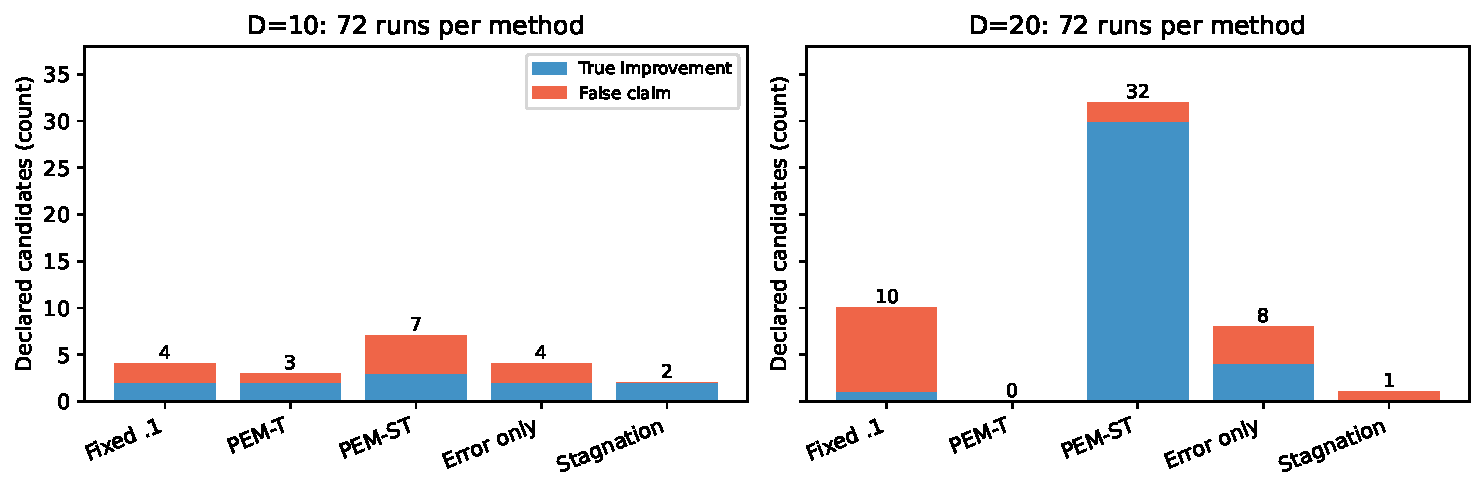
\includegraphics{../cmc_latex_submission/figures/supp_figure_1.pdf}
\caption{Counts of actual improvement and false claims on declared candidates. A zero column denotes no declarations, not an established reliability advantage.}
\end{figure}

Figure S1 exposes both the rarity and composition of improvement declarations. PEM-T makes only three declarations in dimension 10 and none in dimension 20, whereas PEM-ST and the fixed controls produce larger declared subsets. Blue and orange segments distinguish realized improvements from false claims. A missing bar therefore represents an empty conditional sample, while a tall orange segment identifies a declaration rule whose apparent candidates often fail to improve the incumbent.

Failure-only feedback is less detrimental than full feedback on the endpoint summary but still does not achieve an overall benefit over fixed .1. Its combined removal of width and stagnation cannot isolate those terms' independent contributions.

\hypertarget{s1.2-common-history-diagnostics}{%
\subsubsection{S1.2 Common-history diagnostics}\label{s1.2-common-history-diagnostics}}

Table S2 uses the same T bound within each frozen history/model/pool. Under fixed .3 histories, failures at the actually selected point exceed pool failures. Under greedy histories, their ordering reverses. The observation supports history-dependent differences among monitoring objects and does not support a universal direction of selection-induced undercoverage. Each dimension/history has 288 frozen states; each state contributes one actually selected candidate, 256 pool candidates, and 26 top-10\% candidates.

\begin{longtable}[]{@{}lllll@{}}
\caption{Temporal bounds across monitoring objects}\tabularnewline
\toprule\noalign{}
D & History & Pool & Top 10\% & Actually selected \\
\midrule\noalign{}
\endfirsthead
\toprule\noalign{}
D & History & Pool & Top 10\% & Actually selected \\
\midrule\noalign{}
\endhead
\bottomrule\noalign{}
\endlastfoot
10 & fixed03 & 0.0425 & 0.0290 & 0.1250 \\
10 & greedy & 0.1070 & 0.0395 & 0.0868 \\
10 & pool\_random & 0.0773 & 0.0944 & 0.0521 \\
20 & fixed03 & 0.0481 & 0.0423 & 0.1424 \\
20 & greedy & 0.1691 & 0.0843 & 0.0938 \\
20 & pool\_random & 0.0935 & 0.1062 & 0.1042 \\
\end{longtable}

Failure fractions for the selected candidate, full pool, and predicted top 10\% are compared in Figure S2.

\begin{figure}
\centering
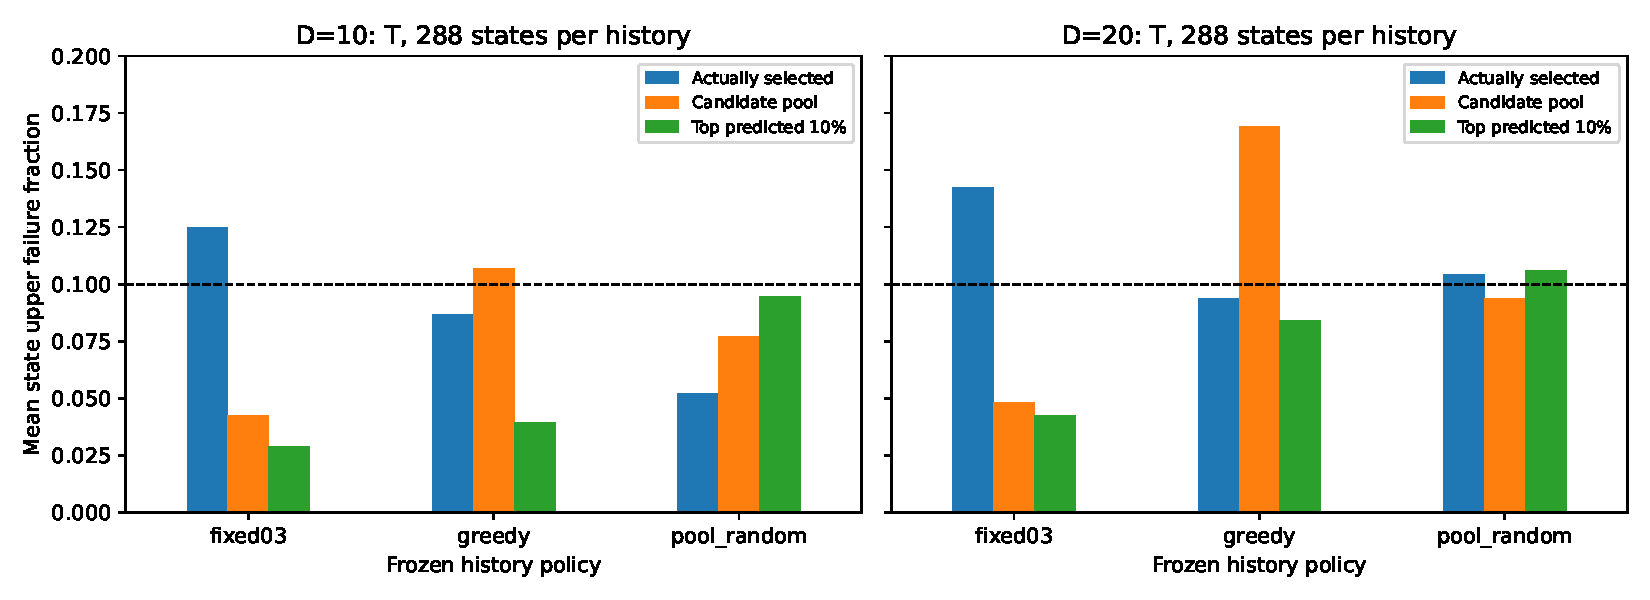
\includegraphics{../cmc_latex_submission/figures/supp_figure_2.pdf}
\caption{State-averaged one-sided failure fractions under frozen common histories. The dashed target is .1. Pool labels are correlated and are not treated as independent problems.}
\end{figure}

Figure S2 compares three monitored objects at identical frozen states: the actually selected candidate, the entire candidate pool, and the top 10\% by predicted value. Under fixed03 histories, the selected-candidate bar is highest; under greedy histories, the pool and top-10\% bars become higher. The dashed 0.1 line is crossed in different directions across histories, which supports reporting the monitored object and its generating policy together.

Table S3 compares calibrators on the actually selected points, with the three histories equally weighted. Spatial localization lowers some diagnostic losses and margins; this is a common-history estimation result, not a closed-loop optimization gain or a coverage guarantee. Approximately one quarter of the dimension-10 checkpoint states fall back because of support, whereas these dimension-20 checkpoints do not.

\begin{longtable}[]{@{}llllll@{}}
\caption{Calibrators on actually selected points}\tabularnewline
\toprule\noalign{}
D & Calibrator & Quantile loss & Margin & ESS & Fallback \\
\midrule\noalign{}
\endfirsthead
\toprule\noalign{}
D & Calibrator & Quantile loss & Margin & ESS & Fallback \\
\midrule\noalign{}
\endhead
\bottomrule\noalign{}
\endlastfoot
10 & G & 0.1355 & 1.1044 & 45.5000 & 0.0000 \\
10 & S & 0.1241 & 0.9463 & 38.8140 & 0.2500 \\
10 & ST & 0.1187 & 0.9175 & 32.1634 & 0.2500 \\
10 & T & 0.1284 & 1.0262 & 37.7288 & 0.2500 \\
20 & G & 0.1465 & 0.9365 & 74.7500 & 0.0000 \\
20 & S & 0.1322 & 0.7874 & 60.5382 & 0.0000 \\
20 & ST & 0.1307 & 0.7643 & 42.6863 & 0.0000 \\
20 & T & 0.1409 & 0.9114 & 52.3172 & 0.0000 \\
\end{longtable}

Pool-declaration subsets are also sparse: T has only 13 declared candidates under dimension-10 fixed .3 histories, and one under dimension-20 fixed .3 histories. Full state, nonempty-state, candidate, and failure denominators are publicly retained in the diagnostic CSV files. Stable reliability is not inferred from a small or empty subset.

\hypertarget{s1.3-common-state-immediate-utility}{%
\subsubsection{S1.3 Common-state immediate utility}\label{s1.3-common-state-immediate-utility}}

Table S4 reports normalized true improvement at one chosen candidate from the same frozen pool. T upper-bound selection is identical to mean greedy and is not repeated as an independent column. Full feedback has lower mean immediate improvement than mean greedy and than the predeclared fixed .3 rule in all six dimension/history cells.

\begin{longtable}[]{@{}lllll@{}}
\caption{Common-state normalized one-step improvement}\tabularnewline
\toprule\noalign{}
D & History & Mean & Fixed .3 & Feedback \\
\midrule\noalign{}
\endfirsthead
\toprule\noalign{}
D & History & Mean & Fixed .3 & Feedback \\
\midrule\noalign{}
\endhead
\bottomrule\noalign{}
\endlastfoot
10 & fixed03 & 0.0260 & 0.0219 & 0.0213 \\
10 & greedy & 0.0310 & 0.0257 & 0.0251 \\
10 & pool\_random & 0.1240 & 0.0925 & 0.0867 \\
20 & fixed03 & 0.0350 & 0.0238 & 0.0172 \\
20 & greedy & 0.0541 & 0.0433 & 0.0381 \\
20 & pool\_random & 0.1326 & 0.0871 & 0.0795 \\
\end{longtable}

Immediate utility does not exclude a delayed benefit from exploration; however, the closed-loop development experiment supplies no evidence of that benefit for this prototype. It is therefore unsupported to state that additional distance exploration repaired the model.

\hypertarget{s2-independent-validation-diagnostics-and-external-references}{%
\section{S2 Independent validation diagnostics and external references}\label{s2-independent-validation-diagnostics-and-external-references}}

\hypertarget{s2.1-history-declarations-and-effective-support}{%
\subsection{S2.1 History, declarations, and effective support}\label{s2.1-history-declarations-and-effective-support}}

The history-interaction estimates are D=10: +0.0851 (Holm p=0.00149); D=20: +0.1225 (Holm p=0.00065); D=40: +0.1449 (Holm p=0.00170). This is the fixed .3 selected-minus-pool difference minus the greedy corresponding difference. Across policies, identical seeds do not imply identical candidate pools. These differences describe the coupled history/policy system rather than a fixed-pool causal effect.

\begin{longtable}[]{@{}llll@{}}
\caption{Temporal pool and actually selected failure fractions, under the prespecified state/run/instance/function aggregation.}\tabularnewline
\toprule\noalign{}
D & History & Pool failure & Selected failure \\
\midrule\noalign{}
\endfirsthead
\toprule\noalign{}
D & History & Pool failure & Selected failure \\
\midrule\noalign{}
\endhead
\bottomrule\noalign{}
\endlastfoot
10 & fixed03 & 0.0479 & 0.1215 \\
10 & greedy & 0.1018 & 0.0903 \\
10 & pool\_random & 0.0859 & 0.0660 \\
20 & fixed03 & 0.0442 & 0.0833 \\
20 & greedy & 0.1494 & 0.0660 \\
20 & pool\_random & 0.0900 & 0.0729 \\
40 & fixed03 & 0.0505 & 0.0799 \\
40 & greedy & 0.1850 & 0.0694 \\
40 & pool\_random & 0.0978 & 0.0694 \\
\end{longtable}

The corresponding selected-minus-pool contrasts are shown in Figure S3.

\begin{figure}
\centering
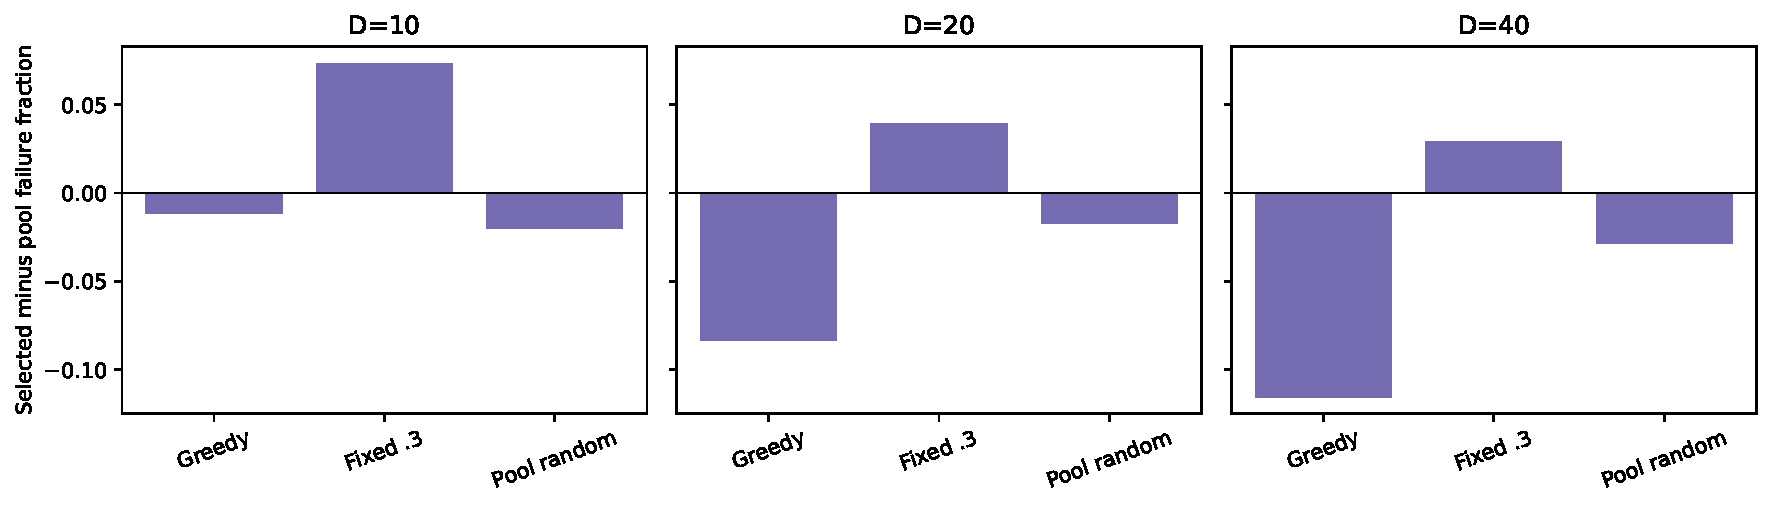
\includegraphics{../cmc_latex_submission/figures/supp_figure_3.pdf}
\caption{Selected-minus-pool failures by preselected history. A reversal is retained rather than interpreted as universal selection deterioration.}
\end{figure}

Figure S3 expresses the same comparison as a signed difference (selected minus pool). Fixed03 bars are positive and greedy bars are negative in every dimension; random-pool bars stay nearer zero. The repeated sign reversal demonstrates that selected-point coverage cannot be summarized independently of the history-generating policy.

\begin{longtable}[]{@{}lllllll@{}}
\caption{Exploration, failures, and declaration denominators in independent closed-loop runs. FDP is pooled false/claims; no-claim FDP is NA.}\tabularnewline
\toprule\noalign{}
D & Method & Exploration & Failure & Claims & False & Pooled FDP \\
\midrule\noalign{}
\endfirsthead
\toprule\noalign{}
D & Method & Exploration & Failure & Claims & False & Pooled FDP \\
\midrule\noalign{}
\endhead
\bottomrule\noalign{}
\endlastfoot
10 & PEM\_ST & 0.3936 & 0.1052 & 48 & 23 & 0.4792 \\
10 & PEM\_T & 0.3967 & 0.1008 & 31 & 20 & 0.6452 \\
10 & fixed01 & 0.0949 & 0.0812 & 35 & 21 & 0.6000 \\
20 & PEM\_ST & 0.3687 & 0.1078 & 158 & 36 & 0.2278 \\
20 & PEM\_T & 0.3644 & 0.0942 & 34 & 27 & 0.7941 \\
20 & fixed01 & 0.1018 & 0.0833 & 48 & 32 & 0.6667 \\
40 & PEM\_ST & 0.3701 & 0.1196 & 870 & 98 & 0.1126 \\
40 & PEM\_T & 0.3435 & 0.0964 & 155 & 30 & 0.1935 \\
40 & fixed01 & 0.1007 & 0.0930 & 388 & 71 & 0.1830 \\
\end{longtable}

For PEM-T, D=10: 31 declarations, 20 false, pooled FDP 64.5\%; D=20: 34 declarations, 27 false, pooled FDP 79.4\%; D=40: 155 declarations, 30 false, pooled FDP 19.4\%. An approximately .1 overall failure fraction does not imply an approximately .1 false-declaration fraction. These small declaration denominators do not establish stable per-declaration probabilities. ST lowers the descriptive selected-point quantile loss in all nine dimension/history cells, yet its closed-loop endpoint remains worse than fixed .1 in every dimension. These are separate diagnostic and trajectory comparisons, not an identified causal relationship.

\begin{longtable}[]{@{}llll@{}}
\caption{Descriptive state-mean support across the three preselected history policies and four checkpoints.}\tabularnewline
\toprule\noalign{}
D & Calibrator & State mean ESS & State mean fallback \\
\midrule\noalign{}
\endfirsthead
\toprule\noalign{}
D & Calibrator & State mean ESS & State mean fallback \\
\midrule\noalign{}
\endhead
\bottomrule\noalign{}
\endlastfoot
10 & ST & 32.9284 & 0.2500 \\
10 & T & 37.7288 & 0.2500 \\
20 & ST & 43.6167 & 0.0000 \\
20 & T & 52.3172 & 0.0000 \\
40 & ST & 49.4855 & 0.0004 \\
40 & T & 58.5602 & 0.0000 \\
\end{longtable}

Temporal and spatiotemporal effective support across checkpoint order is shown in Figure S4.

\begin{figure}
\centering
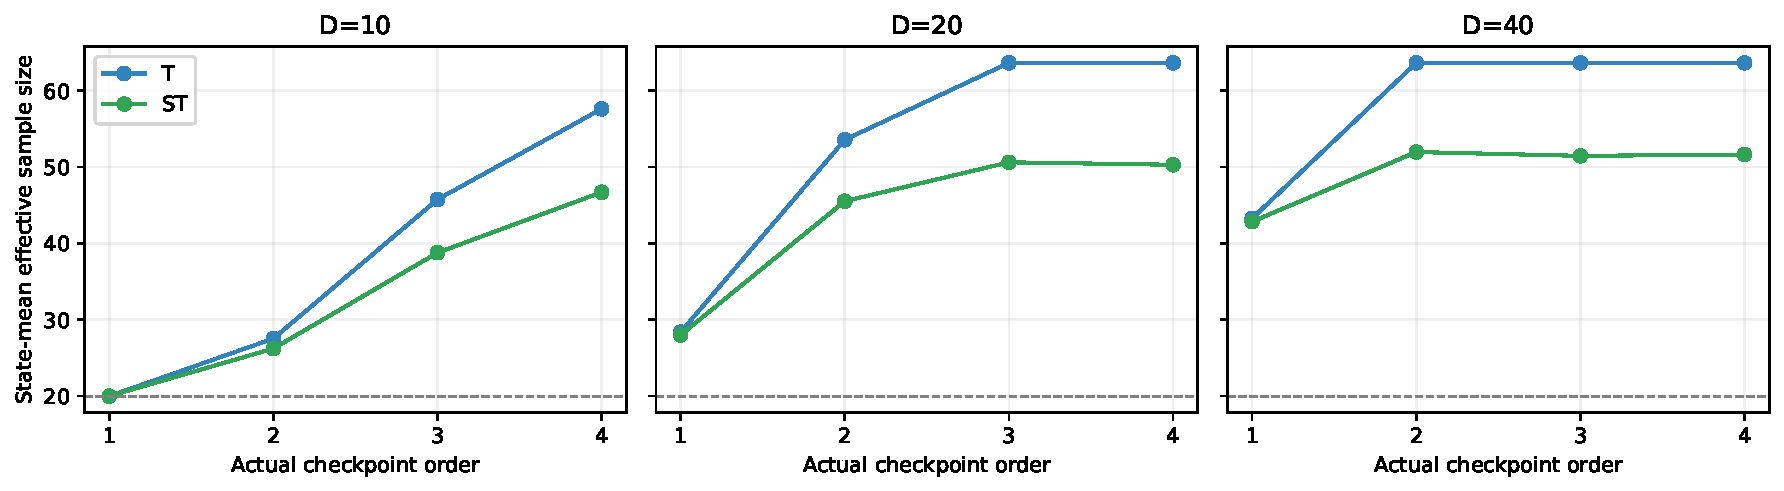
\includegraphics{../cmc_latex_submission/figures/supp_figure_4.pdf}
\caption{T/ST effective support at the four actual checkpoint orders. The threshold is an engineering guard and does not guarantee coverage.}
\end{figure}

Figure S4 shows that effective support grows with checkpoint order for both temporal (T) and spatiotemporal (ST) weighting. T retains more effective observations than ST after localization, and the gap is largest in dimensions 20 and 40. Both curves remain above the support guard after the earliest checkpoint, but the plateaus emphasize that passing the guard is a numerical eligibility condition rather than evidence of calibrated coverage.

The first diagnostic checkpoints are 41/100, 61/200, and 101/400. Sparse declared-pool subsets disclose nonempty states, candidate counts, and failures separately. Localized quantile-loss, margin, ESS, and fallback differences and the five fixed BBOB structure groups are available in full secondary tables; no favorable subgroup is promoted to a primary result.

\hypertarget{s2.2-external-background-references}{%
\subsection{S2.2 External background references}\label{s2.2-external-background-references}}

Sobol and pycma CMA-ES retain their own search mechanisms and initialization. Their 1,296 runs and 302,400 paid evaluations passed separate journal audits. For descriptive common-scale comparison only, each external run's final error is divided by the matching internal common-initialization error, and medians are taken after this run-level normalization. The external optimizers never receive those internal labels. This supports budget-matched background comparison, not a same-history causal comparison or reproduction of published SAEA competitors.

\begin{longtable}[]{@{}llllll@{}}
\caption{Descriptive background endpoint scores over all 24 functions. Lower is better; no additional test family is introduced.}\tabularnewline
\toprule\noalign{}
D & Fixed .1 & PEM-T & PEM-ST & Sobol & CMA-ES \\
\midrule\noalign{}
\endfirsthead
\toprule\noalign{}
D & Fixed .1 & PEM-T & PEM-ST & Sobol & CMA-ES \\
\midrule\noalign{}
\endhead
\bottomrule\noalign{}
\endlastfoot
10 & -0.8823 & -0.7156 & -0.7465 & -0.0805 & -0.4275 \\
20 & -0.8761 & -0.7763 & -0.7877 & -0.1066 & -0.4799 \\
40 & -0.7934 & -0.7295 & -0.7041 & -0.1029 & -0.4440 \\
\end{longtable}

GP-EI and author TuRBO use separate frozen protocols and strict pre-call budget guards. Their complete audited outcomes are now included in the main article. Author-code restart counterexamples are control-flow checks, not performance observations. Resource precheck instances are excluded from every benchmark table.

\hypertarget{s3-complete-bbob-references-and-exclusive-resource-evidence}{%
\section{S3 Complete BBOB references and exclusive resource evidence}\label{s3-complete-bbob-references-and-exclusive-resource-evidence}}

\hypertarget{s3.1-full-descriptive-bbob-reference-evidence}{%
\subsection{S3.1 Full descriptive BBOB reference evidence}\label{s3.1-full-descriptive-bbob-reference-evidence}}

Both frozen GP-EI and author TuRBO-1 batches complete 648 runs and 151,200 paid evaluations each, without reducing functions, repeats, GP training, or acquisition candidates. Together with the six internal and two basic references, all ten methods include 6,480 runs and 1,512,000 paid evaluations. External methods retain their own search and initialization. The matching internal initial-error denominator enters analysis only; normalization precedes within-instance medians. The 24 function scores are equally weighted. These descriptive comparisons add no significance family and do not reproduce the unavailable SAEA competitors.

GP-EI implements classical expected improvement {[}3{]} using the explicitly frozen kernel and search; it is not an exact reproduction of original EGO software. TuRBO-1 uses the author local trust-region implementation {[}25{]} with an external paid-call guard.

\begin{longtable}[]{@{}lrrr@{}}
\caption{Full ten-method function-mean log-relative endpoint scores. Lower is better.}\tabularnewline
\toprule\noalign{}
Method & D=10 & D=20 & D=40 \\
\midrule\noalign{}
\endfirsthead
\toprule\noalign{}
Method & D=10 & D=20 & D=40 \\
\midrule\noalign{}
\endhead
\bottomrule\noalign{}
\endlastfoot
greedy & -0.9152 & -0.9014 & -0.8158 \\
fixed01 & -0.8823 & -0.8761 & -0.7934 \\
fixed03 & -0.7829 & -0.771 & -0.7097 \\
pool\_random & -0.1683 & -0.2223 & -0.2623 \\
PEM\_T & -0.7156 & -0.7763 & -0.7295 \\
PEM\_ST & -0.7465 & -0.7877 & -0.7041 \\
sobol & -0.0805 & -0.1066 & -0.1029 \\
cma\_es & -0.4275 & -0.4799 & -0.444 \\
gp\_ei & -1.3292 & -1.033 & -0.9323 \\
turbo\_1 & -1.102 & -1.1219 & -1.0389 \\
\end{longtable}

The complete ten-method BBOB endpoint comparison is shown in Figure S5.

\begin{figure}
\centering
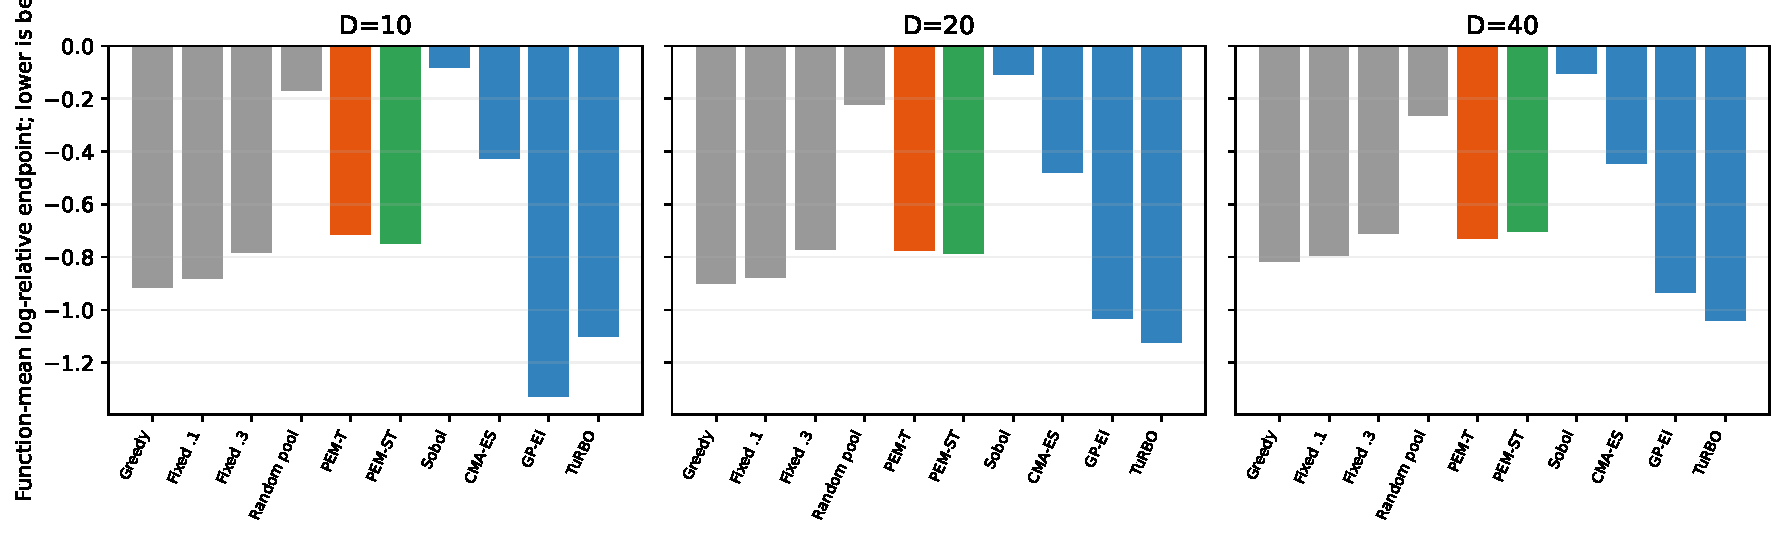
\includegraphics{../cmc_latex_submission/figures/supp_figure_5.pdf}
\caption{Complete BBOB background reference endpoints; no partial runs or resource-precheck instances.}
\end{figure}

Figure S5 retains the full ten-method ordering in each dimension. TuRBO-1 and GP-EI occupy different positions across dimensions, while Sobol remains close to zero and the internal methods form a tighter negative-error group. The panel-wise variation supports use of these methods as descriptive context; it does not justify a cross-protocol causal ranking because their initialization and search mechanisms differ.

\hypertarget{s3.2-exclusive-cost-evidence}{%
\subsection{S3.2 Exclusive cost evidence}\label{s3.2-exclusive-cost-evidence}}

The frozen resource design contains 54 fresh, serial process measurements on f1/instance4 across D=10/20/40 and three repeats of six methods. Their 12,600 paid calls are reported as cost observations, excluded from benchmark effect estimation. Actual process and background-CPU guards precede measurements. Runtime includes journaling and each method retains its own initialization. Greedy/fixed controls still perform temporal monitoring, so these are implemented-system costs, not stripped-down ideal algorithm costs.

\begin{longtable}[]{@{}
  >{\raggedright\arraybackslash}p{(\columnwidth - 8\tabcolsep) * \real{0.1333}}
  >{\raggedleft\arraybackslash}p{(\columnwidth - 8\tabcolsep) * \real{0.2000}}
  >{\raggedleft\arraybackslash}p{(\columnwidth - 8\tabcolsep) * \real{0.2400}}
  >{\raggedleft\arraybackslash}p{(\columnwidth - 8\tabcolsep) * \real{0.1600}}
  >{\raggedleft\arraybackslash}p{(\columnwidth - 8\tabcolsep) * \real{0.2667}}@{}}
\caption{D=10; three-run medians; full min/max and per-process observations remain in the supplement CSV.}\tabularnewline
\toprule\noalign{}
\begin{minipage}[b]{\linewidth}\raggedright
Method
\end{minipage} & \begin{minipage}[b]{\linewidth}\raggedleft
Algorithm s
\end{minipage} & \begin{minipage}[b]{\linewidth}\raggedleft
Nonobjective s
\end{minipage} & \begin{minipage}[b]{\linewidth}\raggedleft
Peak GiB
\end{minipage} & \begin{minipage}[b]{\linewidth}\raggedleft
Post-init prep s
\end{minipage} \\
\midrule\noalign{}
\endfirsthead
\toprule\noalign{}
\begin{minipage}[b]{\linewidth}\raggedright
Method
\end{minipage} & \begin{minipage}[b]{\linewidth}\raggedleft
Algorithm s
\end{minipage} & \begin{minipage}[b]{\linewidth}\raggedleft
Nonobjective s
\end{minipage} & \begin{minipage}[b]{\linewidth}\raggedleft
Peak GiB
\end{minipage} & \begin{minipage}[b]{\linewidth}\raggedleft
Post-init prep s
\end{minipage} \\
\midrule\noalign{}
\endhead
\bottomrule\noalign{}
\endlastfoot
PEM\_ST & 0.6547 & 0.6543 & 0.0945 & 0.0108 \\
PEM\_T & 0.6075 & 0.6072 & 0.0947 & 0.01 \\
fixed01 & 0.602 & 0.6016 & 0.0947 & 0.0099 \\
gp\_ei & 27.6737 & 27.6724 & 0.2863 & 0.3456 \\
greedy & 0.5983 & 0.5979 & 0.0945 & 0.0098 \\
turbo\_1 & 7.4536 & 7.4522 & 0.3905 & 0.0923 \\
\end{longtable}

\begin{longtable}[]{@{}
  >{\raggedright\arraybackslash}p{(\columnwidth - 8\tabcolsep) * \real{0.1333}}
  >{\raggedleft\arraybackslash}p{(\columnwidth - 8\tabcolsep) * \real{0.2000}}
  >{\raggedleft\arraybackslash}p{(\columnwidth - 8\tabcolsep) * \real{0.2400}}
  >{\raggedleft\arraybackslash}p{(\columnwidth - 8\tabcolsep) * \real{0.1600}}
  >{\raggedleft\arraybackslash}p{(\columnwidth - 8\tabcolsep) * \real{0.2667}}@{}}
\caption{D=20; three-run medians; full min/max and per-process observations remain in the supplement CSV.}\tabularnewline
\toprule\noalign{}
\begin{minipage}[b]{\linewidth}\raggedright
Method
\end{minipage} & \begin{minipage}[b]{\linewidth}\raggedleft
Algorithm s
\end{minipage} & \begin{minipage}[b]{\linewidth}\raggedleft
Nonobjective s
\end{minipage} & \begin{minipage}[b]{\linewidth}\raggedleft
Peak GiB
\end{minipage} & \begin{minipage}[b]{\linewidth}\raggedleft
Post-init prep s
\end{minipage} \\
\midrule\noalign{}
\endfirsthead
\toprule\noalign{}
\begin{minipage}[b]{\linewidth}\raggedright
Method
\end{minipage} & \begin{minipage}[b]{\linewidth}\raggedleft
Algorithm s
\end{minipage} & \begin{minipage}[b]{\linewidth}\raggedleft
Nonobjective s
\end{minipage} & \begin{minipage}[b]{\linewidth}\raggedleft
Peak GiB
\end{minipage} & \begin{minipage}[b]{\linewidth}\raggedleft
Post-init prep s
\end{minipage} \\
\midrule\noalign{}
\endhead
\bottomrule\noalign{}
\endlastfoot
PEM\_ST & 1.6909 & 1.6901 & 0.0946 & 0.012 \\
PEM\_T & 1.5254 & 1.5246 & 0.0948 & 0.0108 \\
fixed01 & 1.5252 & 1.5244 & 0.0948 & 0.0108 \\
gp\_ei & 175.864 & 175.861 & 0.3059 & 1.0989 \\
greedy & 1.5246 & 1.5238 & 0.0945 & 0.0108 \\
turbo\_1 & 35.0159 & 35.013 & 0.5936 & 0.2183 \\
\end{longtable}

\begin{longtable}[]{@{}
  >{\raggedright\arraybackslash}p{(\columnwidth - 8\tabcolsep) * \real{0.1333}}
  >{\raggedleft\arraybackslash}p{(\columnwidth - 8\tabcolsep) * \real{0.2000}}
  >{\raggedleft\arraybackslash}p{(\columnwidth - 8\tabcolsep) * \real{0.2400}}
  >{\raggedleft\arraybackslash}p{(\columnwidth - 8\tabcolsep) * \real{0.1600}}
  >{\raggedleft\arraybackslash}p{(\columnwidth - 8\tabcolsep) * \real{0.2667}}@{}}
\caption{D=40; three-run medians; full min/max and per-process observations remain in the supplement CSV.}\tabularnewline
\toprule\noalign{}
\begin{minipage}[b]{\linewidth}\raggedright
Method
\end{minipage} & \begin{minipage}[b]{\linewidth}\raggedleft
Algorithm s
\end{minipage} & \begin{minipage}[b]{\linewidth}\raggedleft
Nonobjective s
\end{minipage} & \begin{minipage}[b]{\linewidth}\raggedleft
Peak GiB
\end{minipage} & \begin{minipage}[b]{\linewidth}\raggedleft
Post-init prep s
\end{minipage} \\
\midrule\noalign{}
\endfirsthead
\toprule\noalign{}
\begin{minipage}[b]{\linewidth}\raggedright
Method
\end{minipage} & \begin{minipage}[b]{\linewidth}\raggedleft
Algorithm s
\end{minipage} & \begin{minipage}[b]{\linewidth}\raggedleft
Nonobjective s
\end{minipage} & \begin{minipage}[b]{\linewidth}\raggedleft
Peak GiB
\end{minipage} & \begin{minipage}[b]{\linewidth}\raggedleft
Post-init prep s
\end{minipage} \\
\midrule\noalign{}
\endhead
\bottomrule\noalign{}
\endlastfoot
PEM\_ST & 4.7496 & 4.7476 & 0.096 & 0.0157 \\
PEM\_T & 4.3878 & 4.3856 & 0.0962 & 0.0145 \\
fixed01 & 4.3787 & 4.3766 & 0.0965 & 0.0145 \\
gp\_ei & 1308.81 & 1308.8 & 0.3073 & 4.0897 \\
greedy & 4.3615 & 4.3594 & 0.0958 & 0.0144 \\
turbo\_1 & 255.912 & 255.906 & 1.0791 & 0.7993 \\
\end{longtable}

The measured-overhead and assumed-objective-cost scenarios are shown in Figure S6.

\begin{figure}
\centering
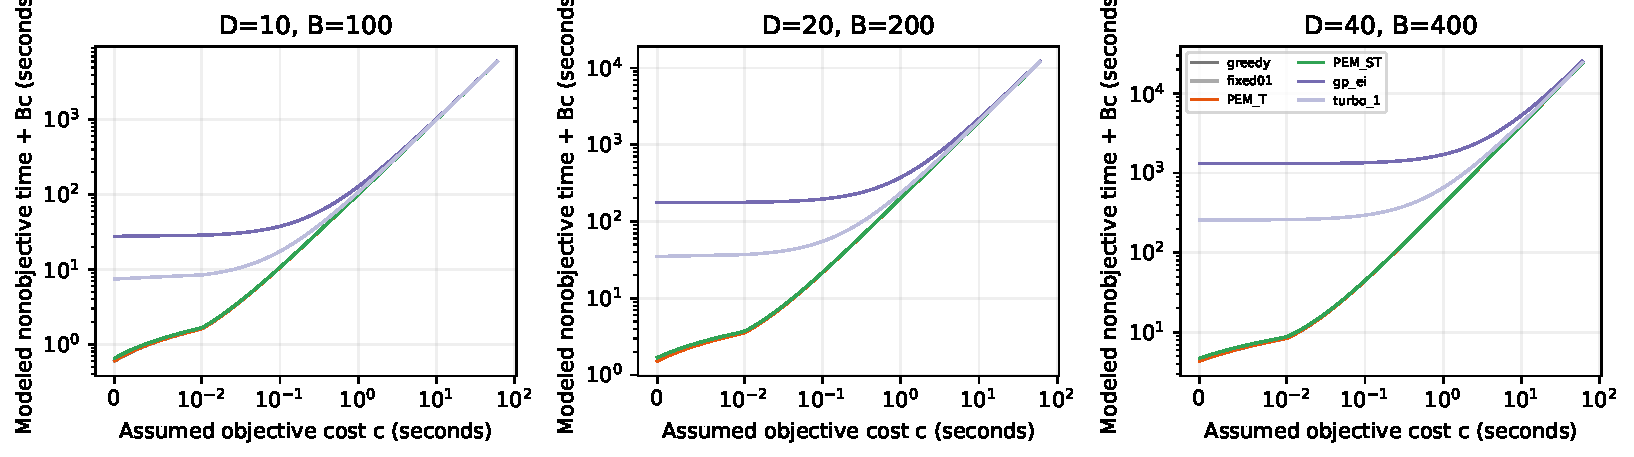
\includegraphics{../cmc_latex_submission/figures/supp_figure_6.pdf}
\caption{Hypothetical objective-cost scenarios from serial measurements; all methods use the same B in a dimension.}
\end{figure}

Figure S6 separates measured algorithm overhead from an assumed per-evaluation objective cost. The left side of each log-scale panel is dominated by method overhead, which is largest for GP-EI and TuRBO-1. As objective cost increases, all lines approach the common slope imposed by the identical evaluation budget. The intersections mark cost regimes in which overhead ceases to dominate; they are scenario calculations, not measured parallel speedups.

At an assumed objective cost c, total time is modeled as measured nonobjective time plus Bc. This scenario is not an observed application acceleration. Equal evaluation budgets have equal objective-cost slopes and cannot establish evaluation savings.

\hypertarget{s4-lassobench-application-transfer}{%
\section{S4 LassoBench application transfer}\label{s4-lassobench-application-transfer}}

\hypertarget{s4.1-lassobench-mechanism-transfer}{%
\subsection{S4.1 LassoBench mechanism transfer}\label{s4.1-lassobench-mechanism-transfer}}

LassoBench {[}24{]} provides the application objectives. A separate protocol is frozen before formal seed42 labels. Three original tasks (D=60/100/180), eight methods, twenty optimization repeats, and 500 evaluations yield 480 runs and 240,000 full configuration evaluations (1,200,000 CV-fold solves). Internal initialization is 140/220/380 paid calls; external initialization remains native. The author five-fold full-fidelity objective, fixed data/splits, solver settings, bounds, and target definitions are unchanged.

Unknown optimum is never imputed. The main endpoint is original validation loss. After all 500 labels are saved, the first lowest-validation configuration receives exactly one author test call, adding 480 single fits separately. Synthetic test MSPE uses the author fixed oracle normalizer, while DNA uses absolute test MSE; these scales are not pooled. The synthetic constructor computes its fixed test normalizer, but no test-performance result enters any optimization feedback.

\begin{longtable}[]{@{}
  >{\raggedright\arraybackslash}p{(\columnwidth - 10\tabcolsep) * \real{0.1299}}
  >{\raggedleft\arraybackslash}p{(\columnwidth - 10\tabcolsep) * \real{0.1688}}
  >{\raggedleft\arraybackslash}p{(\columnwidth - 10\tabcolsep) * \real{0.1039}}
  >{\raggedleft\arraybackslash}p{(\columnwidth - 10\tabcolsep) * \real{0.1039}}
  >{\raggedleft\arraybackslash}p{(\columnwidth - 10\tabcolsep) * \real{0.2597}}
  >{\raggedleft\arraybackslash}p{(\columnwidth - 10\tabcolsep) * \real{0.2338}}@{}}
\caption{synt\_simple; twenty optimization-run dispersion and post-completion test medians.}\tabularnewline
\toprule\noalign{}
\begin{minipage}[b]{\linewidth}\raggedright
Method
\end{minipage} & \begin{minipage}[b]{\linewidth}\raggedleft
CV median
\end{minipage} & \begin{minipage}[b]{\linewidth}\raggedleft
Q1
\end{minipage} & \begin{minipage}[b]{\linewidth}\raggedleft
Q3
\end{minipage} & \begin{minipage}[b]{\linewidth}\raggedleft
Test MSPE median
\end{minipage} & \begin{minipage}[b]{\linewidth}\raggedleft
F-score median
\end{minipage} \\
\midrule\noalign{}
\endfirsthead
\toprule\noalign{}
\begin{minipage}[b]{\linewidth}\raggedright
Method
\end{minipage} & \begin{minipage}[b]{\linewidth}\raggedleft
CV median
\end{minipage} & \begin{minipage}[b]{\linewidth}\raggedleft
Q1
\end{minipage} & \begin{minipage}[b]{\linewidth}\raggedleft
Q3
\end{minipage} & \begin{minipage}[b]{\linewidth}\raggedleft
Test MSPE median
\end{minipage} & \begin{minipage}[b]{\linewidth}\raggedleft
F-score median
\end{minipage} \\
\midrule\noalign{}
\endhead
\bottomrule\noalign{}
\endlastfoot
PEM\_ST & 0.7896 & 0.7656 & 0.8528 & 1.1435 & 0.6667 \\
PEM\_T & 0.7714 & 0.7557 & 0.8654 & 1.2013 & 0.6667 \\
cma\_es & 0.758 & 0.7176 & 0.7826 & 1.072 & 0.5455 \\
fixed01 & 0.7534 & 0.7092 & 0.816 & 1.1441 & 0.6667 \\
gp\_ei & 1.0118 & 0.9392 & 1.0847 & 1.1167 & 0.6 \\
greedy & 0.7501 & 0.703 & 0.7755 & 1.1078 & 0.6 \\
sobol & 1.2057 & 1.0326 & 1.2544 & 1.1865 & 0.4808 \\
turbo\_1 & 0.6448 & 0.5888 & 0.7032 & 1.0643 & 0.6 \\
\end{longtable}

\begin{longtable}[]{@{}
  >{\raggedright\arraybackslash}p{(\columnwidth - 10\tabcolsep) * \real{0.1299}}
  >{\raggedleft\arraybackslash}p{(\columnwidth - 10\tabcolsep) * \real{0.1688}}
  >{\raggedleft\arraybackslash}p{(\columnwidth - 10\tabcolsep) * \real{0.1039}}
  >{\raggedleft\arraybackslash}p{(\columnwidth - 10\tabcolsep) * \real{0.1039}}
  >{\raggedleft\arraybackslash}p{(\columnwidth - 10\tabcolsep) * \real{0.2597}}
  >{\raggedleft\arraybackslash}p{(\columnwidth - 10\tabcolsep) * \real{0.2338}}@{}}
\caption{synt\_medium; twenty optimization-run dispersion and post-completion test medians.}\tabularnewline
\toprule\noalign{}
\begin{minipage}[b]{\linewidth}\raggedright
Method
\end{minipage} & \begin{minipage}[b]{\linewidth}\raggedleft
CV median
\end{minipage} & \begin{minipage}[b]{\linewidth}\raggedleft
Q1
\end{minipage} & \begin{minipage}[b]{\linewidth}\raggedleft
Q3
\end{minipage} & \begin{minipage}[b]{\linewidth}\raggedleft
Test MSPE median
\end{minipage} & \begin{minipage}[b]{\linewidth}\raggedleft
F-score median
\end{minipage} \\
\midrule\noalign{}
\endfirsthead
\toprule\noalign{}
\begin{minipage}[b]{\linewidth}\raggedright
Method
\end{minipage} & \begin{minipage}[b]{\linewidth}\raggedleft
CV median
\end{minipage} & \begin{minipage}[b]{\linewidth}\raggedleft
Q1
\end{minipage} & \begin{minipage}[b]{\linewidth}\raggedleft
Q3
\end{minipage} & \begin{minipage}[b]{\linewidth}\raggedleft
Test MSPE median
\end{minipage} & \begin{minipage}[b]{\linewidth}\raggedleft
F-score median
\end{minipage} \\
\midrule\noalign{}
\endhead
\bottomrule\noalign{}
\endlastfoot
PEM\_ST & 1.146 & 1.1122 & 1.1731 & 0.7697 & 0.7692 \\
PEM\_T & 1.1519 & 1.1327 & 1.1684 & 0.7562 & 0.8013 \\
cma\_es & 1.1888 & 1.1345 & 1.237 & 0.7927 & 0.625 \\
fixed01 & 1.1186 & 1.0751 & 1.1418 & 0.7486 & 0.7692 \\
gp\_ei & 1.61 & 1.5226 & 1.7486 & 0.8469 & 0.6667 \\
greedy & 1.1103 & 1.069 & 1.1616 & 0.7703 & 0.7692 \\
sobol & 1.8953 & 1.7099 & 2.0302 & 0.8846 & 0.625 \\
turbo\_1 & 1.0277 & 0.9575 & 1.0632 & 0.835 & 0.625 \\
\end{longtable}

\begin{longtable}[]{@{}
  >{\raggedright\arraybackslash}p{(\columnwidth - 10\tabcolsep) * \real{0.1299}}
  >{\raggedleft\arraybackslash}p{(\columnwidth - 10\tabcolsep) * \real{0.1688}}
  >{\raggedleft\arraybackslash}p{(\columnwidth - 10\tabcolsep) * \real{0.1039}}
  >{\raggedleft\arraybackslash}p{(\columnwidth - 10\tabcolsep) * \real{0.1039}}
  >{\raggedleft\arraybackslash}p{(\columnwidth - 10\tabcolsep) * \real{0.2597}}
  >{\raggedright\arraybackslash}p{(\columnwidth - 10\tabcolsep) * \real{0.2338}}@{}}
\caption{DNA; twenty optimization-run dispersion and post-completion test medians.}\tabularnewline
\toprule\noalign{}
\begin{minipage}[b]{\linewidth}\raggedright
Method
\end{minipage} & \begin{minipage}[b]{\linewidth}\raggedleft
CV median
\end{minipage} & \begin{minipage}[b]{\linewidth}\raggedleft
Q1
\end{minipage} & \begin{minipage}[b]{\linewidth}\raggedleft
Q3
\end{minipage} & \begin{minipage}[b]{\linewidth}\raggedleft
Test MSPE median
\end{minipage} & \begin{minipage}[b]{\linewidth}\raggedright
F-score median
\end{minipage} \\
\midrule\noalign{}
\endfirsthead
\toprule\noalign{}
\begin{minipage}[b]{\linewidth}\raggedright
Method
\end{minipage} & \begin{minipage}[b]{\linewidth}\raggedleft
CV median
\end{minipage} & \begin{minipage}[b]{\linewidth}\raggedleft
Q1
\end{minipage} & \begin{minipage}[b]{\linewidth}\raggedleft
Q3
\end{minipage} & \begin{minipage}[b]{\linewidth}\raggedleft
Test MSPE median
\end{minipage} & \begin{minipage}[b]{\linewidth}\raggedright
F-score median
\end{minipage} \\
\midrule\noalign{}
\endhead
\bottomrule\noalign{}
\endlastfoot
PEM\_ST & 0.3071 & 0.3056 & 0.3092 & 0.3304 & NA \\
PEM\_T & 0.3073 & 0.3054 & 0.3093 & 0.3277 & NA \\
cma\_es & 0.3014 & 0.2992 & 0.3043 & 0.3285 & NA \\
fixed01 & 0.306 & 0.3025 & 0.3079 & 0.3307 & NA \\
gp\_ei & 0.336 & 0.3328 & 0.3384 & 0.3495 & NA \\
greedy & 0.3057 & 0.3042 & 0.3067 & 0.327 & NA \\
sobol & 0.3348 & 0.332 & 0.3375 & 0.3439 & NA \\
turbo\_1 & 0.3028 & 0.3005 & 0.3052 & 0.3278 & NA \\
\end{longtable}

\begin{longtable}[]{@{}
  >{\raggedright\arraybackslash}p{(\columnwidth - 14\tabcolsep) * \real{0.1477}}
  >{\raggedleft\arraybackslash}p{(\columnwidth - 14\tabcolsep) * \real{0.2386}}
  >{\raggedleft\arraybackslash}p{(\columnwidth - 14\tabcolsep) * \real{0.1250}}
  >{\raggedleft\arraybackslash}p{(\columnwidth - 14\tabcolsep) * \real{0.1250}}
  >{\raggedleft\arraybackslash}p{(\columnwidth - 14\tabcolsep) * \real{0.1136}}
  >{\raggedleft\arraybackslash}p{(\columnwidth - 14\tabcolsep) * \real{0.0909}}
  >{\raggedleft\arraybackslash}p{(\columnwidth - 14\tabcolsep) * \real{0.0795}}
  >{\raggedleft\arraybackslash}p{(\columnwidth - 14\tabcolsep) * \real{0.0795}}@{}}
\caption{Prespecified application family, PEM-T minus fixed .1 raw final validation loss. Positive favors the fixed control. Intervals are unadjusted paired-run bootstrap.}\tabularnewline
\toprule\noalign{}
\begin{minipage}[b]{\linewidth}\raggedright
Task
\end{minipage} & \begin{minipage}[b]{\linewidth}\raggedleft
Median difference
\end{minipage} & \begin{minipage}[b]{\linewidth}\raggedleft
CI low
\end{minipage} & \begin{minipage}[b]{\linewidth}\raggedleft
CI high
\end{minipage} & \begin{minipage}[b]{\linewidth}\raggedleft
Holm p
\end{minipage} & \begin{minipage}[b]{\linewidth}\raggedleft
Loss
\end{minipage} & \begin{minipage}[b]{\linewidth}\raggedleft
Win
\end{minipage} & \begin{minipage}[b]{\linewidth}\raggedleft
Tie
\end{minipage} \\
\midrule\noalign{}
\endfirsthead
\toprule\noalign{}
\begin{minipage}[b]{\linewidth}\raggedright
Task
\end{minipage} & \begin{minipage}[b]{\linewidth}\raggedleft
Median difference
\end{minipage} & \begin{minipage}[b]{\linewidth}\raggedleft
CI low
\end{minipage} & \begin{minipage}[b]{\linewidth}\raggedleft
CI high
\end{minipage} & \begin{minipage}[b]{\linewidth}\raggedleft
Holm p
\end{minipage} & \begin{minipage}[b]{\linewidth}\raggedleft
Loss
\end{minipage} & \begin{minipage}[b]{\linewidth}\raggedleft
Win
\end{minipage} & \begin{minipage}[b]{\linewidth}\raggedleft
Tie
\end{minipage} \\
\midrule\noalign{}
\endhead
\bottomrule\noalign{}
\endlastfoot
synt\_simple & 0.0503 & 0.0032 & 0.0725 & 0.0826 & 14 & 6 & 0 \\
synt\_medium & 0.0393 & 0.0221 & 0.0626 & 0.0192 & 16 & 4 & 0 \\
DNA & 0.0027 & 0.0005279 & 0.0044 & 0.0592 & 16 & 4 & 0 \\
\end{longtable}

synt\_simple: higher, Holm p=0.0826; synt\_medium: higher, Holm p=0.0192; DNA: higher, Holm p=0.0592.

The three comparisons form an application-only Holm family, separate from the nine BBOB mechanism tests. Twenty repeats describe optimization randomness on one fixed dataset and split per task, not twenty independent datasets. The Wilcoxon and paired bootstrap assumptions and limits are retained regardless of significance or direction.

Original-scale validation endpoints for the three LassoBench tasks are shown in Figure S7.

\begin{figure}
\centering
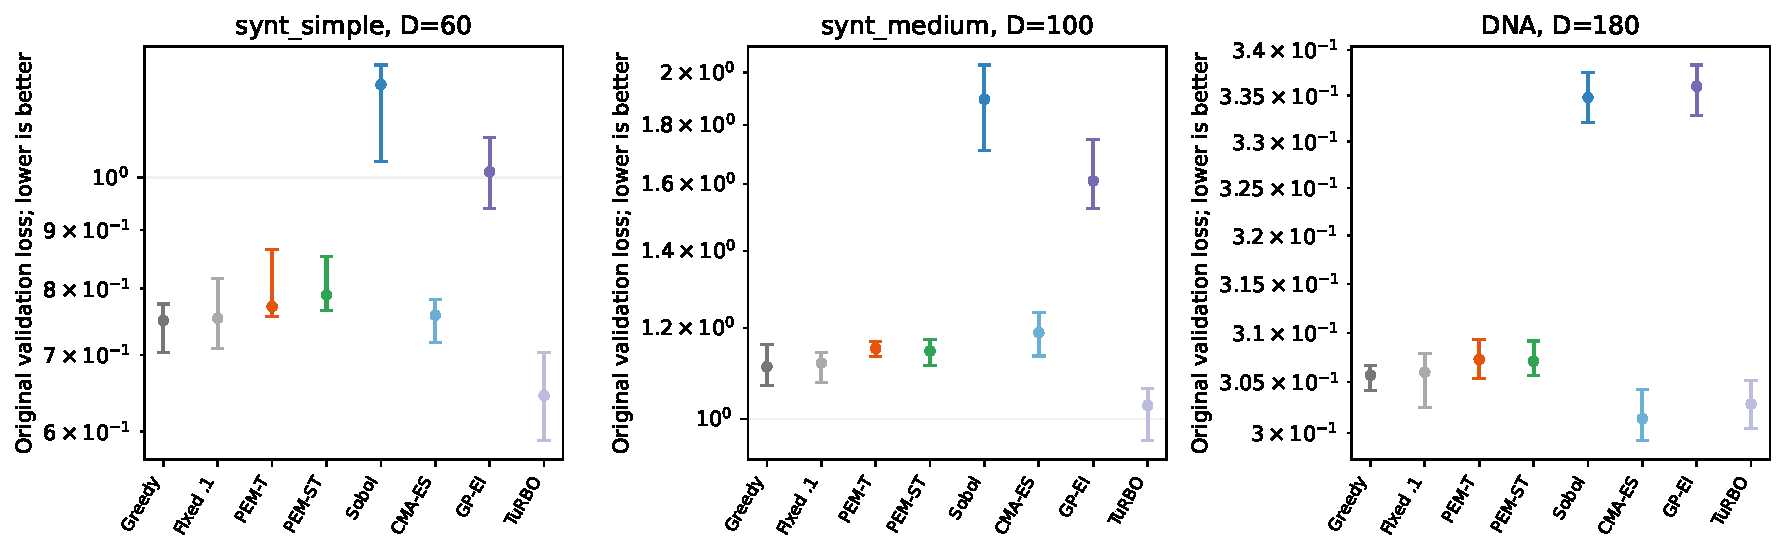
\includegraphics{../cmc_latex_submission/figures/supp_figure_7.pdf}
\caption{Application original validation endpoints with run-IQR bars; unknown-optimum error is never constructed.}
\end{figure}

Figure S7 reports the original validation loss on its native scale for each LassoBench task. The synt\_simple and synt\_medium panels separate the lower-loss internal and trust-region methods from Sobol and GP-EI, whereas the DNA panel compresses most methods into a narrow band. The run-interquartile bars reveal substantial dispersion for the weaker synthetic-task endpoints and discourage conclusions based only on median rank.

Their median and interquartile convergence histories are shown in Figure S8.

\begin{figure}
\centering
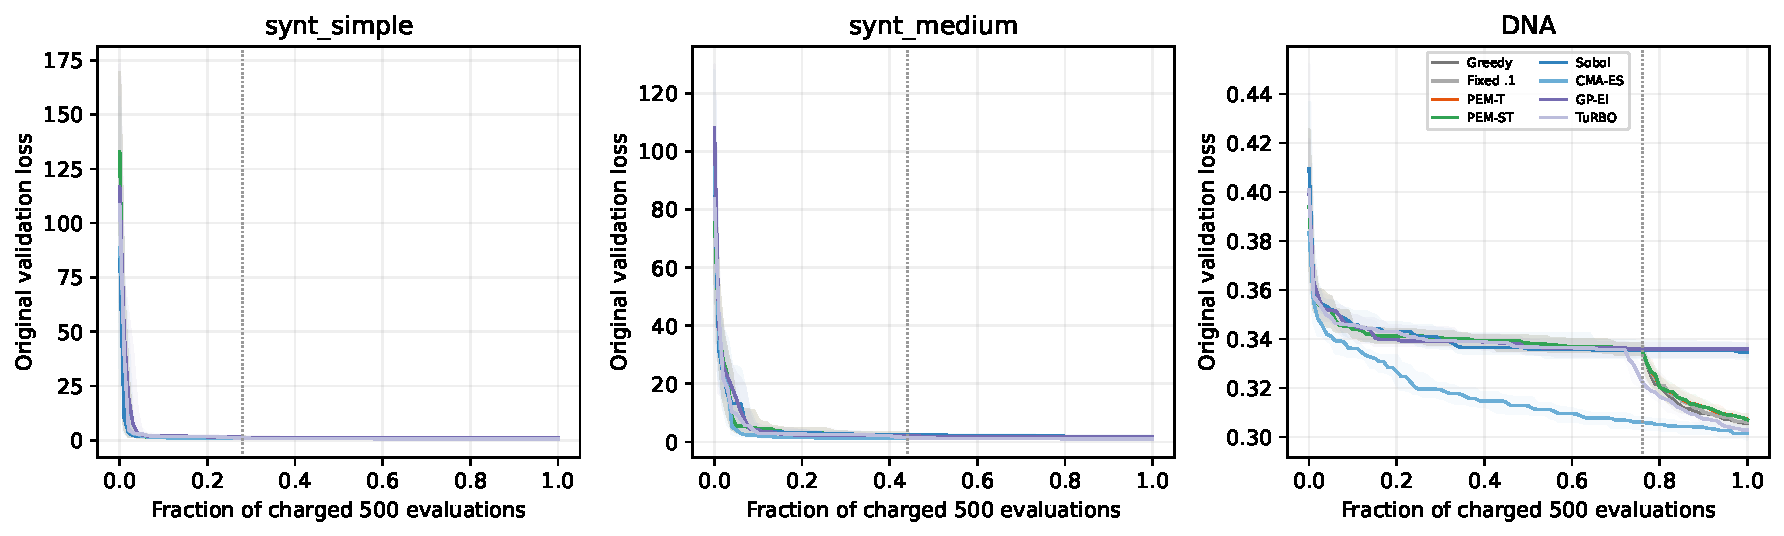
\includegraphics{../cmc_latex_submission/figures/supp_figure_8.pdf}
\caption{Application original-loss median and IQR curves. The dotted line marks internal initialization; external designs differ. Zero fraction displays the first paid label.}
\end{figure}

Figure S8 shows how the endpoint differences arise. Most improvement on the two synthetic tasks occurs early, followed by long plateaus, while DNA retains smaller and more gradual changes. The dotted initialization boundary applies to the internal configurations only; external curves begin from their native designs. The figure is therefore used to describe timing and stability, not to claim identical starting conditions.

\begin{longtable}[]{@{}
  >{\raggedright\arraybackslash}p{(\columnwidth - 14\tabcolsep) * \real{0.1383}}
  >{\raggedright\arraybackslash}p{(\columnwidth - 14\tabcolsep) * \real{0.1064}}
  >{\raggedleft\arraybackslash}p{(\columnwidth - 14\tabcolsep) * \real{0.1170}}
  >{\raggedleft\arraybackslash}p{(\columnwidth - 14\tabcolsep) * \real{0.1064}}
  >{\raggedleft\arraybackslash}p{(\columnwidth - 14\tabcolsep) * \real{0.1064}}
  >{\raggedleft\arraybackslash}p{(\columnwidth - 14\tabcolsep) * \real{0.0957}}
  >{\raggedright\arraybackslash}p{(\columnwidth - 14\tabcolsep) * \real{0.1489}}
  >{\raggedleft\arraybackslash}p{(\columnwidth - 14\tabcolsep) * \real{0.1809}}@{}}
\caption{Descriptive post-initialization selected-point monitoring; no hidden pool objectives are acquired.}\tabularnewline
\toprule\noalign{}
\begin{minipage}[b]{\linewidth}\raggedright
Task
\end{minipage} & \begin{minipage}[b]{\linewidth}\raggedright
Method
\end{minipage} & \begin{minipage}[b]{\linewidth}\raggedleft
Failure
\end{minipage} & \begin{minipage}[b]{\linewidth}\raggedleft
Q-loss
\end{minipage} & \begin{minipage}[b]{\linewidth}\raggedleft
Claims
\end{minipage} & \begin{minipage}[b]{\linewidth}\raggedleft
False
\end{minipage} & \begin{minipage}[b]{\linewidth}\raggedright
Pooled FDP
\end{minipage} & \begin{minipage}[b]{\linewidth}\raggedleft
No-claim runs
\end{minipage} \\
\midrule\noalign{}
\endfirsthead
\toprule\noalign{}
\begin{minipage}[b]{\linewidth}\raggedright
Task
\end{minipage} & \begin{minipage}[b]{\linewidth}\raggedright
Method
\end{minipage} & \begin{minipage}[b]{\linewidth}\raggedleft
Failure
\end{minipage} & \begin{minipage}[b]{\linewidth}\raggedleft
Q-loss
\end{minipage} & \begin{minipage}[b]{\linewidth}\raggedleft
Claims
\end{minipage} & \begin{minipage}[b]{\linewidth}\raggedleft
False
\end{minipage} & \begin{minipage}[b]{\linewidth}\raggedright
Pooled FDP
\end{minipage} & \begin{minipage}[b]{\linewidth}\raggedleft
No-claim runs
\end{minipage} \\
\midrule\noalign{}
\endhead
\bottomrule\noalign{}
\endlastfoot
DNA & PEM\_ST & 0.0704 & 0.0698 & 0 & 0 & NA & 20 \\
DNA & PEM\_T & 0.0629 & 0.084 & 0 & 0 & NA & 20 \\
DNA & fixed01 & 0.0346 & 0.0627 & 0 & 0 & NA & 20 \\
DNA & greedy & 0.0079 & 0.041 & 1 & 1 & 1.0000 & 19 \\
synt\_medium & PEM\_ST & 0.1036 & 0.0778 & 53 & 46 & 0.8679 & 1 \\
synt\_medium & PEM\_T & 0.0887 & 0.0904 & 7 & 6 & 0.8571 & 14 \\
synt\_medium & fixed01 & 0.0505 & 0.0452 & 27 & 23 & 0.8519 & 5 \\
synt\_medium & greedy & 0.0134 & 0.0147 & 60 & 54 & 0.9000 & 1 \\
synt\_simple & PEM\_ST & 0.1103 & 0.0946 & 75 & 74 & 0.9867 & 1 \\
synt\_simple & PEM\_T & 0.0931 & 0.1104 & 7 & 6 & 0.8571 & 15 \\
synt\_simple & fixed01 & 0.0549 & 0.0476 & 76 & 74 & 0.9737 & 1 \\
synt\_simple & greedy & 0.0367 & 0.0137 & 220 & 218 & 0.9909 & 0 \\
\end{longtable}

These closed-loop histories differ between methods and do not identify same-pool causal effects. Zero declarations give NA FDP, with counts disclosed. The 300-dimensional synt\_high extension therefore uses its separately frozen 1,000-evaluation protocol, reported in Section S5. Application findings cannot undo the failed original development gate.

\hypertarget{s5-predefined-300-dimensional-extension}{%
\section{S5 Predefined 300-dimensional extension}\label{s5-predefined-300-dimensional-extension}}

The predefined synt\_high extension used 1,000 paid evaluations because the unchanged internal initialization requires 620, exceeding the 500-evaluation primary-application budget. Eight methods completed 20 optimization runs on one fixed seed42 data set and split (160 runs; 160,000 validation evaluations; 800,000 CV-fold solves), followed by exactly one held-out test call per completed run. The low-effective-dimensional synthetic construction and different budget preclude a general high-dimensional or cross-task superiority claim.

\hypertarget{s5.1-endpoints-and-convergence}{%
\subsection{S5.1 Endpoints and convergence}\label{s5.1-endpoints-and-convergence}}

\begin{longtable}[]{@{}
  >{\raggedright\arraybackslash}p{(\columnwidth - 6\tabcolsep) * \real{0.0990}}
  >{\raggedright\arraybackslash}p{(\columnwidth - 6\tabcolsep) * \real{0.2970}}
  >{\raggedright\arraybackslash}p{(\columnwidth - 6\tabcolsep) * \real{0.2871}}
  >{\raggedright\arraybackslash}p{(\columnwidth - 6\tabcolsep) * \real{0.3168}}@{}}
\toprule\noalign{}
\begin{minipage}[b]{\linewidth}\raggedright
Method
\end{minipage} & \begin{minipage}[b]{\linewidth}\raggedright
Validation median {[}Q1, Q3{]}
\end{minipage} & \begin{minipage}[b]{\linewidth}\raggedright
Test MSPE median {[}Q1, Q3{]}
\end{minipage} & \begin{minipage}[b]{\linewidth}\raggedright
Test F-score median {[}Q1, Q3{]}
\end{minipage} \\
\midrule\noalign{}
\endhead
\bottomrule\noalign{}
\endlastfoot
greedy & 1.38 {[}1.334, 1.435{]} & 1.508 {[}1.466, 1.608{]} & 0.6897 {[}0.6522, 0.7186{]} \\
fixed01 & 1.392 {[}1.345, 1.442{]} & 1.615 {[}1.484, 1.677{]} & 0.6977 {[}0.6596, 0.7317{]} \\
PEM\_T & 1.364 {[}1.338, 1.439{]} & 1.58 {[}1.503, 1.653{]} & 0.7143 {[}0.678, 0.7548{]} \\
PEM\_ST & 1.372 {[}1.312, 1.476{]} & 1.614 {[}1.525, 1.653{]} & 0.6977 {[}0.6818, 0.7317{]} \\
sobol & 18.54 {[}16.12, 22.64{]} & 13.45 {[}10.07, 19.15{]} & 0.3314 {[}0.3055, 0.354{]} \\
cma\_es & 1.145 {[}1.089, 1.179{]} & 1.696 {[}1.612, 1.909{]} & 0.6522 {[}0.6, 0.6667{]} \\
gp\_ei & 17.04 {[}14.89, 21{]} & 13.5 {[}9.747, 19.81{]} & 0.359 {[}0.3123, 0.3709{]} \\
turbo\_1 & 1.157 {[}1.128, 1.265{]} & 1.654 {[}1.6, 1.798{]} & 0.723 {[}0.6977, 0.75{]} \\
\end{longtable}

The 300-dimensional endpoint distribution is shown in Figure S9.

\begin{figure}
\centering
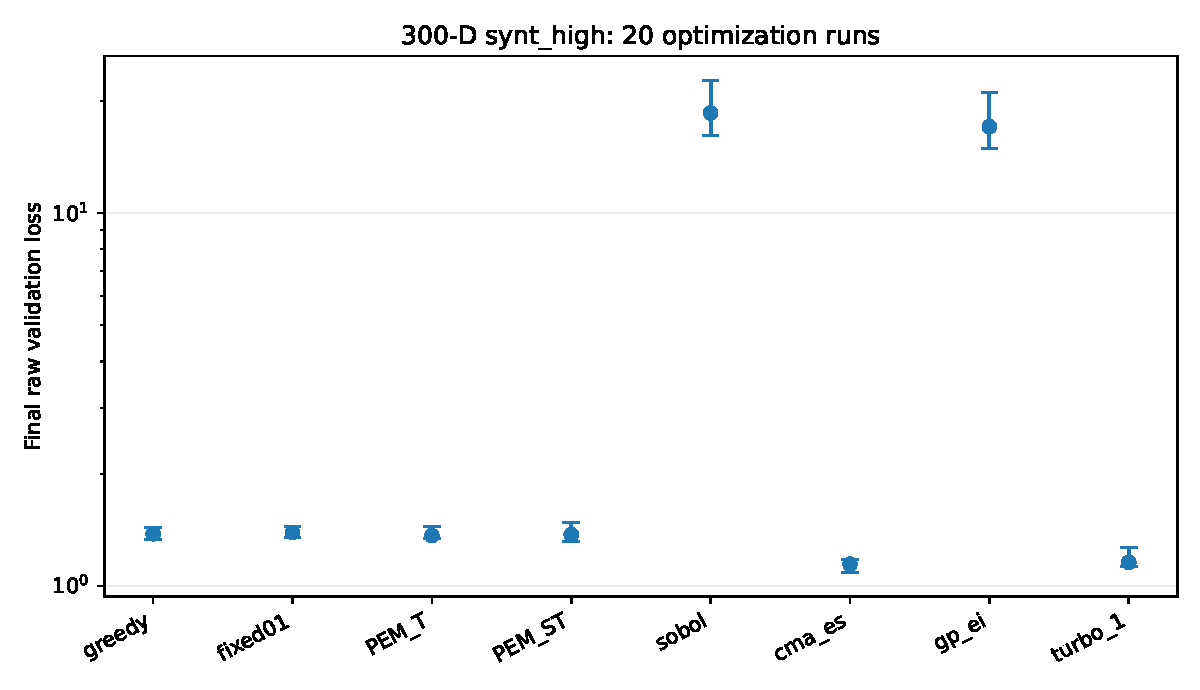
\includegraphics{../cmc_latex_submission/figures/supp_figure_9.pdf}
\caption{High-dimensional endpoints}
\end{figure}

Figure S9 separates the 300-dimensional methods into two endpoint groups. The four internal configurations, CMA-ES, and TuRBO-1 finish near the lower cluster, whereas Sobol and GP-EI remain more than an order of magnitude higher on the logarithmic axis. Interquartile bars are shown for all methods so that the apparent grouping can be assessed against between-run variability.

The associated paid-budget convergence histories are shown in Figure S10.

\begin{figure}
\centering
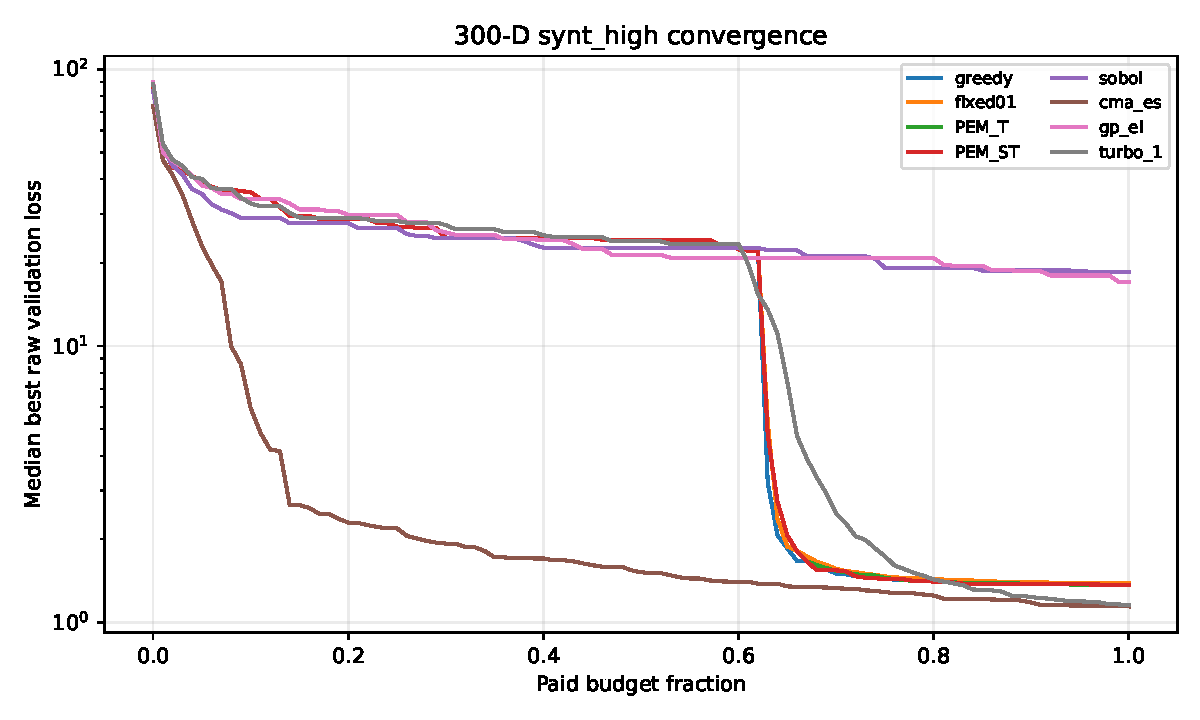
\includegraphics{../cmc_latex_submission/figures/supp_figure_10.pdf}
\caption{High-dimensional convergence}
\end{figure}

Figure S10 reveals distinct routes to the lower endpoint cluster. TuRBO-1 improves early and continuously; the internal methods change sharply only after their long initialization consumes about 62\% of the budget. CMA-ES improves later, while Sobol and GP-EI remain on the upper plateau. This timing difference is why the 1,000-evaluation protocol is reported separately from the primary 500-evaluation application study.

The prespecified descriptive PEM\_T-minus-fixed01 median raw-loss difference was -0.01788, with paired-run bootstrap interval {[}-0.06477, 0.05017{]} and 11/9/0 negative/positive/zero differences. No p-value was computed and this contrast was not added to the three-test primary application family. The interval conditions on one fixed data set and split.

\hypertarget{s5.2-selected-point-feedback-and-resource-boundary}{%
\subsection{S5.2 Selected-point feedback and resource boundary}\label{s5.2-selected-point-feedback-and-resource-boundary}}

\begin{longtable}[]{@{}
  >{\raggedright\arraybackslash}p{(\columnwidth - 12\tabcolsep) * \real{0.1408}}
  >{\raggedleft\arraybackslash}p{(\columnwidth - 12\tabcolsep) * \real{0.1549}}
  >{\raggedleft\arraybackslash}p{(\columnwidth - 12\tabcolsep) * \real{0.1268}}
  >{\raggedleft\arraybackslash}p{(\columnwidth - 12\tabcolsep) * \real{0.1549}}
  >{\raggedleft\arraybackslash}p{(\columnwidth - 12\tabcolsep) * \real{0.1690}}
  >{\raggedleft\arraybackslash}p{(\columnwidth - 12\tabcolsep) * \real{0.1408}}
  >{\raggedleft\arraybackslash}p{(\columnwidth - 12\tabcolsep) * \real{0.1127}}@{}}
\toprule\noalign{}
\begin{minipage}[b]{\linewidth}\raggedright
Method
\end{minipage} & \begin{minipage}[b]{\linewidth}\raggedleft
Failure
\end{minipage} & \begin{minipage}[b]{\linewidth}\raggedleft
QLoss
\end{minipage} & \begin{minipage}[b]{\linewidth}\raggedleft
Explore
\end{minipage} & \begin{minipage}[b]{\linewidth}\raggedleft
Fallback
\end{minipage} & \begin{minipage}[b]{\linewidth}\raggedleft
Claims
\end{minipage} & \begin{minipage}[b]{\linewidth}\raggedleft
FDP
\end{minipage} \\
\midrule\noalign{}
\endhead
\bottomrule\noalign{}
\endlastfoot
greedy & 0.07447 & 0.01695 & 0 & 0 & 257 & 1 \\
fixed01 & 0.07895 & 0.03878 & 0.09618 & 0 & 127 & 0.9921 \\
PEM\_T & 0.08921 & 0.07535 & 0.3405 & 0 & 5 & 1 \\
PEM\_ST & 0.1266 & 0.06124 & 0.3854 & 0.01184 & 119 & 0.9916 \\
\end{longtable}

Feedback summaries cover the 380 post-initialization selections per internal run. They describe each closed-loop history and do not establish same-pool causal effects or conformal error control. Before formal labels, eight separate full-budget resource runs completed 8,000 validation evaluations and zero test calls. Their mixed-load timings supported feasibility only; formal optimization times are reported as observed process costs rather than exclusive speedups.

\hypertarget{s6-prespecified-model-and-training-cap-sensitivity}{%
\section{S6 Prespecified model and training-cap sensitivity}\label{s6-prespecified-model-and-training-cap-sensitivity}}

Five preselected BBOB structure representatives (f1, f6, f10, f15, f20), dimensions 20/40, instances 14--16, and three optimization repeats evaluated PEM\_T under the base setting and four one-factor perturbations. All 450 runs and 135,000 paid evaluations completed; no hidden diagnostic labels or inferential tests were added. This local sensitivity study does not select a replacement default.

\begin{longtable}[]{@{}
  >{\raggedleft\arraybackslash}p{(\columnwidth - 6\tabcolsep) * \real{0.0694}}
  >{\raggedright\arraybackslash}p{(\columnwidth - 6\tabcolsep) * \real{0.1528}}
  >{\raggedright\arraybackslash}p{(\columnwidth - 6\tabcolsep) * \real{0.3889}}
  >{\raggedright\arraybackslash}p{(\columnwidth - 6\tabcolsep) * \real{0.3889}}@{}}
\toprule\noalign{}
\begin{minipage}[b]{\linewidth}\raggedleft
D
\end{minipage} & \begin{minipage}[b]{\linewidth}\raggedright
Variant
\end{minipage} & \begin{minipage}[b]{\linewidth}\raggedright
Endpoint median {[}Q1, Q3{]}
\end{minipage} & \begin{minipage}[b]{\linewidth}\raggedright
AUC median {[}Q1, Q3{]}
\end{minipage} \\
\midrule\noalign{}
\endhead
\bottomrule\noalign{}
\endlastfoot
20 & base & -1.536 {[}-2.168, -0.8568{]} & -0.962 {[}-1.292, -0.5037{]} \\
20 & cap128 & -1.439 {[}-1.903, -0.7494{]} & -0.9267 {[}-1.28, -0.5181{]} \\
20 & cap512 & -1.536 {[}-2.168, -0.8568{]} & -0.962 {[}-1.292, -0.5037{]} \\
20 & scale125 & -1.085 {[}-1.722, -0.6441{]} & -0.6593 {[}-1.087, -0.3838{]} \\
20 & scale500 & -1.473 {[}-2.095, -0.6943{]} & -0.776 {[}-1.079, -0.4353{]} \\
40 & base & -1.275 {[}-1.676, -0.8544{]} & -0.8335 {[}-1.096, -0.5196{]} \\
40 & cap128 & -0.9176 {[}-1.179, -0.5716{]} & -0.6855 {[}-0.8808, -0.4435{]} \\
40 & cap512 & -1.235 {[}-1.69, -0.8008{]} & -0.8185 {[}-1.123, -0.5374{]} \\
40 & scale125 & -0.8456 {[}-1.18, -0.5364{]} & -0.5406 {[}-0.7806, -0.3901{]} \\
40 & scale500 & -1.151 {[}-1.311, -0.7564{]} & -0.7301 {[}-0.9111, -0.4361{]} \\
\end{longtable}

Paired model and training-cap endpoint distributions are shown in Figure S11.

\begin{figure}
\centering
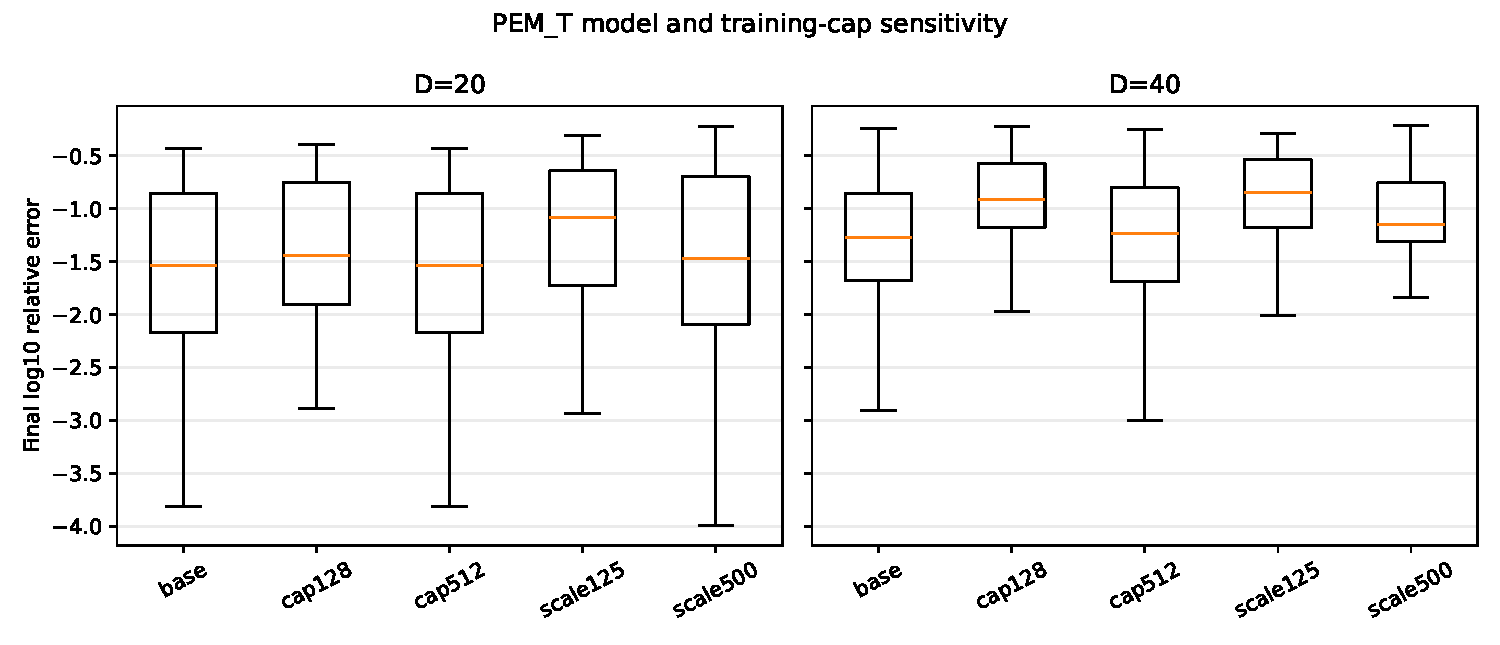
\includegraphics{../cmc_latex_submission/figures/supp_figure_11.pdf}
\caption{Model and training-cap sensitivity}
\end{figure}

Figure S11 displays paired endpoint distributions for the base model, two training caps, and two length-scale variants. Cap512 coincides with the base configuration in dimension 20 because the cap is never reached. Other variants shift the median and spread, especially in dimension 40, but none converts the sensitivity analysis into an unqualified favorable result for the feedback mechanism.

Paired differences below are variant minus base in final log10 relative error. Negative values favor the variant descriptively.

\begin{longtable}[]{@{}
  >{\raggedleft\arraybackslash}p{(\columnwidth - 10\tabcolsep) * \real{0.0641}}
  >{\raggedright\arraybackslash}p{(\columnwidth - 10\tabcolsep) * \real{0.1410}}
  >{\raggedright\arraybackslash}p{(\columnwidth - 10\tabcolsep) * \real{0.3846}}
  >{\raggedleft\arraybackslash}p{(\columnwidth - 10\tabcolsep) * \real{0.1538}}
  >{\raggedleft\arraybackslash}p{(\columnwidth - 10\tabcolsep) * \real{0.1538}}
  >{\raggedleft\arraybackslash}p{(\columnwidth - 10\tabcolsep) * \real{0.1026}}@{}}
\toprule\noalign{}
\begin{minipage}[b]{\linewidth}\raggedleft
D
\end{minipage} & \begin{minipage}[b]{\linewidth}\raggedright
Variant
\end{minipage} & \begin{minipage}[b]{\linewidth}\raggedright
Difference median {[}Q1, Q3{]}
\end{minipage} & \begin{minipage}[b]{\linewidth}\raggedleft
Negative
\end{minipage} & \begin{minipage}[b]{\linewidth}\raggedleft
Positive
\end{minipage} & \begin{minipage}[b]{\linewidth}\raggedleft
Zero
\end{minipage} \\
\midrule\noalign{}
\endhead
\bottomrule\noalign{}
\endlastfoot
20 & cap128 & 0.06854 {[}0, 0.1836{]} & 11 & 30 & 4 \\
20 & cap512 & 0 {[}0, 0{]} & 0 & 0 & 45 \\
20 & scale125 & 0.2805 {[}0.08773, 0.5608{]} & 8 & 37 & 0 \\
20 & scale500 & 0.09344 {[}-0.04563, 0.2851{]} & 14 & 31 & 0 \\
40 & cap128 & 0.3284 {[}0.0957, 0.4718{]} & 4 & 41 & 0 \\
40 & cap512 & 0.005203 {[}-0.02706, 0.08161{]} & 18 & 27 & 0 \\
40 & scale125 & 0.3253 {[}0.03915, 0.656{]} & 8 & 37 & 0 \\
40 & scale500 & 0.09029 {[}-0.002699, 0.2816{]} & 12 & 33 & 0 \\
\end{longtable}

The 45 D=20 base/cap512 pairs had identical PRE/LABEL trajectories and candidate arrays, as neither cap was reached. Thus that equality is an implementation invariant rather than evidence that caps never matter. At D=40, cap512 is untruncated only within this 400-evaluation scope.

\begin{longtable}[]{@{}rlrrrr@{}}
\toprule\noalign{}
D & Variant & Capped & Failure & Explore & Fallback \\
\midrule\noalign{}
\endhead
\bottomrule\noalign{}
\endlastfoot
20 & base & 0 & 0.08746 & 0.2789 & 0 \\
20 & cap128 & 3195 & 0.1332 & 0.3444 & 0 \\
20 & cap512 & 0 & 0.08746 & 0.2789 & 0 \\
20 & scale125 & 0 & 0.1002 & 0.3173 & 0 \\
20 & scale500 & 0 & 0.07175 & 0.283 & 0 \\
40 & base & 6435 & 0.08889 & 0.2541 & 0 \\
40 & cap128 & 12195 & 0.1893 & 0.5487 & 0 \\
40 & cap512 & 0 & 0.08993 & 0.2591 & 0 \\
40 & scale125 & 6435 & 0.09733 & 0.2797 & 0 \\
40 & scale500 & 6435 & 0.08674 & 0.2902 & 0 \\
\end{longtable}

Feedback metrics follow each variant's distinct closed-loop history. The limited function/instance set, shared initialization, and absence of multiplicity-adjusted inference restrict these results to robustness description.

\hypertarget{s7-prespecified-budget-performance-sensitivity-and-recovery-accounting}{%
\section{S7 Prespecified budget-performance sensitivity and recovery accounting}\label{s7-prespecified-budget-performance-sensitivity-and-recovery-accounting}}

\hypertarget{s7.1-design-and-aggregation}{%
\subsection{S7.1 Design and aggregation}\label{s7.1-design-and-aggregation}}

Five prespecified BBOB structure representatives (f1, f6, f10, f15, and f20), dimensions 20/40, instances 17--19, and three repeats were run independently at total budgets 5D, 10D, and 15D. Six internal configurations and four external references completed all 2,700 runs and 810,000 paid evaluations, with no diagnostic labels. Each endpoint uses the matching fixed01 common-initialization error as a post-run denominator. The repeat median is first taken within each function-instance cell; the three instances within each function and the five function scores are then averaged with equal weight. No hypothesis test, confidence interval, or parameter selection was added.

\hypertarget{s7.2-endpoints-and-convergence}{%
\subsection{S7.2 Endpoints and convergence}\label{s7.2-endpoints-and-convergence}}

Lower values are better. Each table entry is the prespecified hierarchical mean final log10 relative error.

\begin{longtable}[]{@{}
  >{\raggedright\arraybackslash}p{(\columnwidth - 12\tabcolsep) * \real{0.1688}}
  >{\raggedleft\arraybackslash}p{(\columnwidth - 12\tabcolsep) * \real{0.1299}}
  >{\raggedleft\arraybackslash}p{(\columnwidth - 12\tabcolsep) * \real{0.1429}}
  >{\raggedleft\arraybackslash}p{(\columnwidth - 12\tabcolsep) * \real{0.1429}}
  >{\raggedleft\arraybackslash}p{(\columnwidth - 12\tabcolsep) * \real{0.1299}}
  >{\raggedleft\arraybackslash}p{(\columnwidth - 12\tabcolsep) * \real{0.1429}}
  >{\raggedleft\arraybackslash}p{(\columnwidth - 12\tabcolsep) * \real{0.1429}}@{}}
\toprule\noalign{}
\begin{minipage}[b]{\linewidth}\raggedright
Method
\end{minipage} & \begin{minipage}[b]{\linewidth}\raggedleft
D20-5D
\end{minipage} & \begin{minipage}[b]{\linewidth}\raggedleft
D20-10D
\end{minipage} & \begin{minipage}[b]{\linewidth}\raggedleft
D20-15D
\end{minipage} & \begin{minipage}[b]{\linewidth}\raggedleft
D40-5D
\end{minipage} & \begin{minipage}[b]{\linewidth}\raggedleft
D40-10D
\end{minipage} & \begin{minipage}[b]{\linewidth}\raggedleft
D40-15D
\end{minipage} \\
\midrule\noalign{}
\endhead
\bottomrule\noalign{}
\endlastfoot
greedy & -0.961 & -1.768 & -2.097 & -0.9999 & -1.544 & -1.643 \\
fixed01 & -0.9322 & -1.749 & -2.035 & -0.9727 & -1.53 & -1.664 \\
fixed03 & -0.6895 & -1.616 & -2.041 & -0.7998 & -1.491 & -1.634 \\
pool\_random & -0.08979 & -0.3369 & -0.433 & -0.187 & -0.3509 & -0.4963 \\
PEM\_T & -0.7538 & -1.689 & -1.987 & -0.8891 & -1.477 & -1.598 \\
PEM\_ST & -0.7407 & -1.676 & -2.039 & -0.8906 & -1.456 & -1.57 \\
sobol & -0.1024 & -0.1513 & -0.209 & -0.0429 & -0.09157 & -0.09792 \\
cma\_es & -0.4835 & -0.7414 & -1.068 & -0.4553 & -0.6883 & -0.949 \\
gp\_ei & -1.642 & -2.388 & -2.574 & -1.651 & -1.993 & -2.174 \\
turbo\_1 & -1.08 & -2.216 & -2.502 & -0.9778 & -1.943 & -2.516 \\
\end{longtable}

Endpoint changes across the three prespecified total budgets are shown in Figure S12.

\begin{figure}
\centering
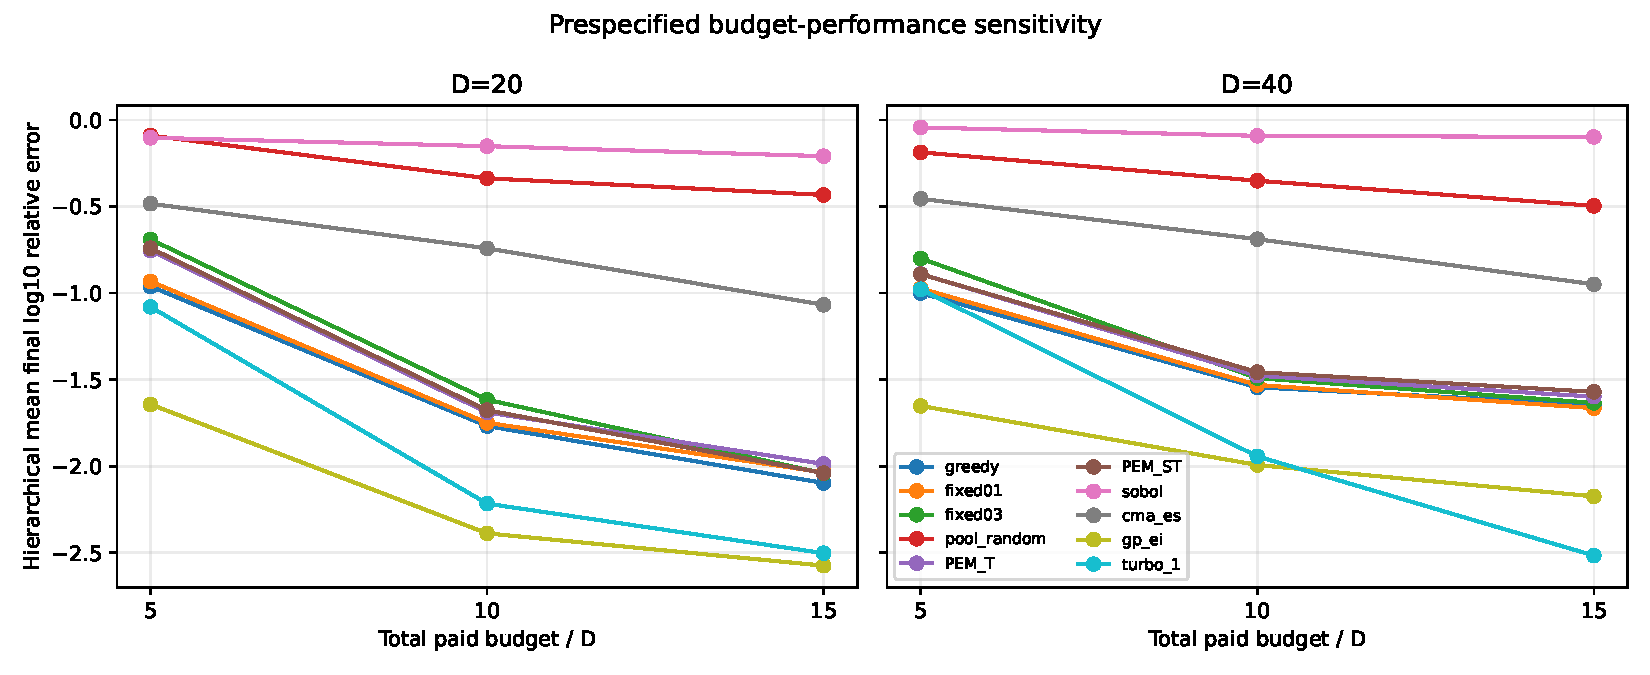
\includegraphics{../cmc_latex_submission/figures/supp_figure_12.pdf}
\caption{Budget-sensitivity endpoints}
\end{figure}

Figure S12 connects endpoint quality to total budget. Most methods improve as the allowance rises from 5D to 15D, but the monitored internal variants remain above the strongest external curves. The slopes differ by dimension, which indicates that additional budget changes the magnitude of the gap without reversing the principal mechanism conclusion.

The corresponding independent-run convergence histories are shown in Figure S13.

\begin{figure}
\centering
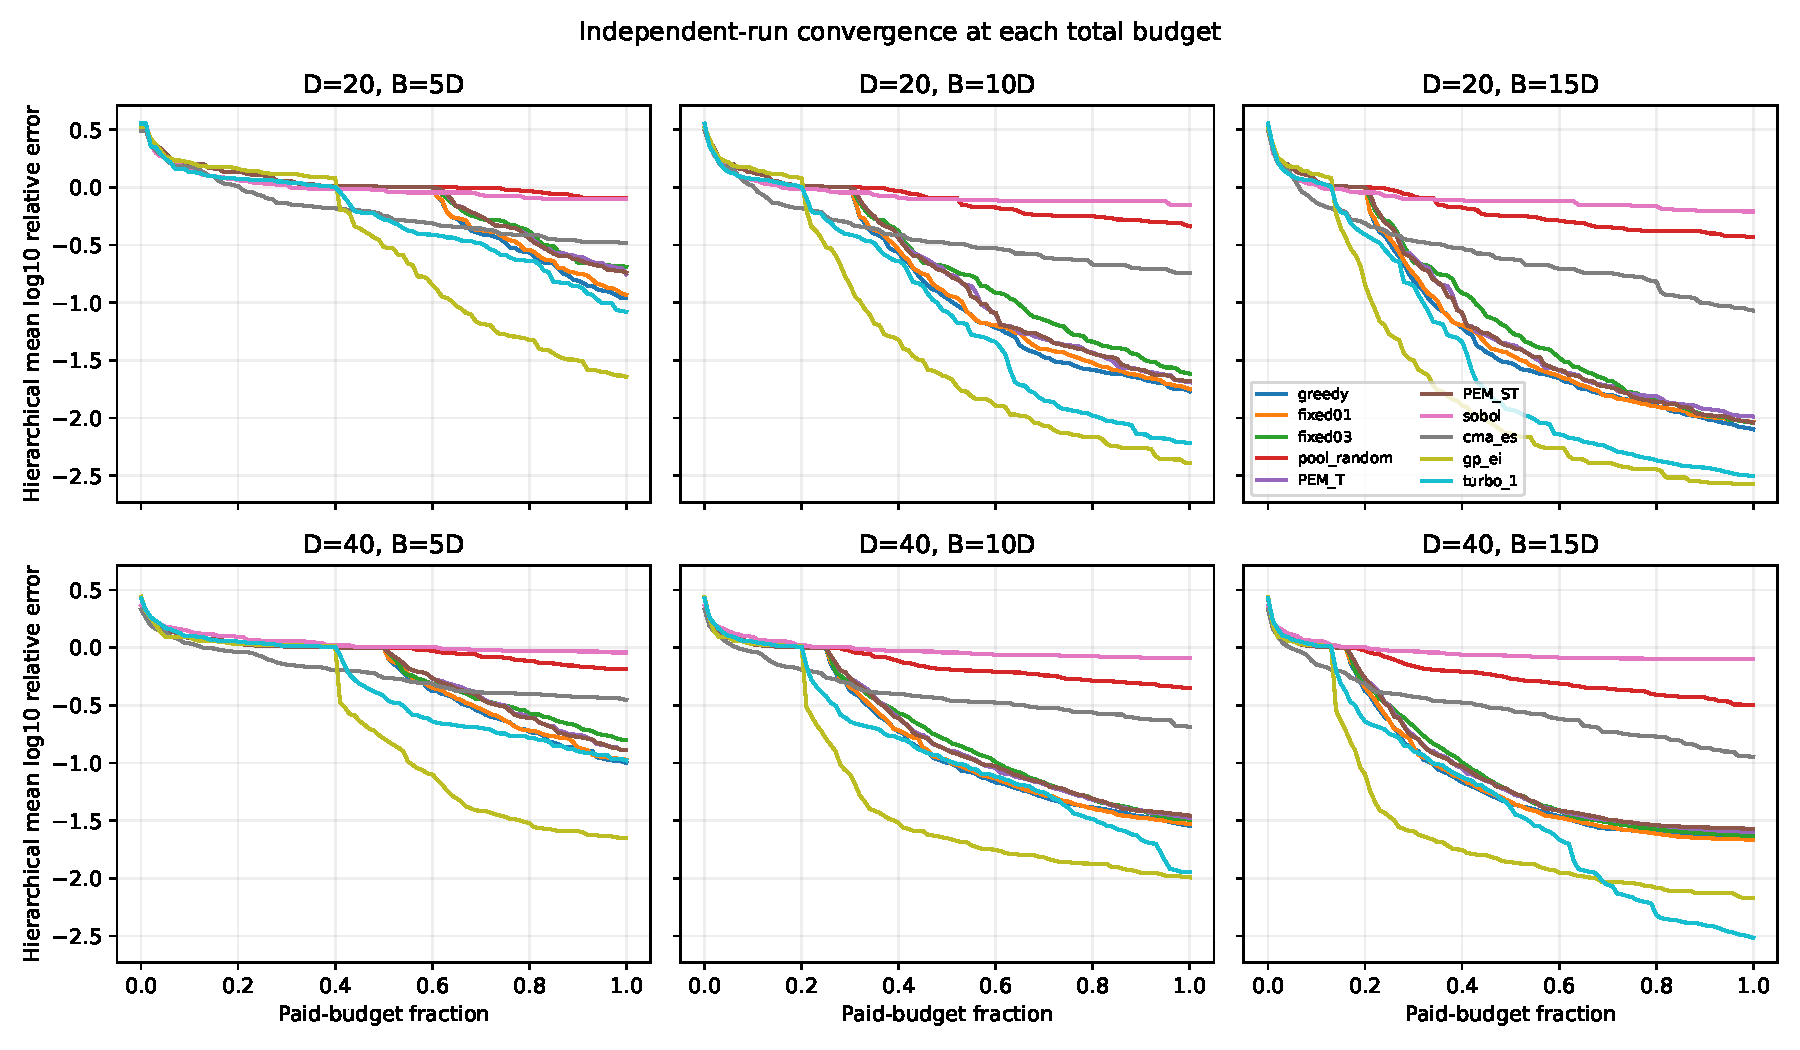
\includegraphics{../cmc_latex_submission/figures/supp_figure_13.pdf}
\caption{Budget-sensitivity convergence}
\end{figure}

Figure S13 plots each independent run against its own paid-budget fraction. The 5D, 10D, and 15D panels share early behavior where the information prefixes are equal, then separate as longer runs acquire additional labels. External methods do not share those internal prefixes. The six panels therefore expose both convergence shape and the information-order boundary used in the recovery audit.

Each budget is a separate optimization run. A longer-budget endpoint therefore supplies robustness evidence under a larger total allowance; it is not a continuation selected after observing the shorter run. The restricted five-function, two-dimension design and descriptive aggregation do not establish a general ranking.

\hypertarget{s7.3-prefix-and-information-order-audit}{%
\subsection{S7.3 Prefix and information-order audit}\label{s7.3-prefix-and-information-order-audit}}

\begin{longtable}[]{@{}lll@{}}
\toprule\noalign{}
Method & Equal 5D/10D/15D prefixes & Required invariant \\
\midrule\noalign{}
\endhead
\bottomrule\noalign{}
\endlastfoot
greedy & 90/90 & yes \\
fixed01 & 90/90 & yes \\
fixed03 & 90/90 & yes \\
pool\_random & 90/90 & yes \\
PEM\_T & 90/90 & yes \\
PEM\_ST & 90/90 & yes \\
sobol & 90/90 & no \\
cma\_es & 90/90 & no \\
gp\_ei & 0/90 & no \\
turbo\_1 & 0/90 & no \\
\end{longtable}

The budget-blind internal core was required to reproduce identical 5D and 10D prefixes inside the corresponding longer run; all 540 required comparisons passed. External prefix equality was recorded rather than required: 180/360 comparisons were equal. That count is an implementation observation, not an assumption used to validate external methods. Full audits replayed all 810,000 PRE/LABEL pairs, internal bounds and management states, and 7,020 raw-file hashes. No total-budget value entered the internal proposal rule.

\hypertarget{s7.4-recovery-accounting-and-evidence-boundary}{%
\subsection{S7.4 Recovery accounting and evidence boundary}\label{s7.4-recovery-accounting-and-evidence-boundary}}

The budget-sensitivity interruption left 8 incomplete units with 1,791 physically acquired labels. Their complete directories were archived before resumption, and each affected unit was rerun from its frozen seed. These labels never entered the 2,700 canonical trajectories. The budget-sensitivity physical ledger is therefore 811,791 calls: 810,000 canonical evaluations plus 1,791 disclosed interrupted-run calls. The additional calls are excluded from endpoints, convergence curves, and algorithm budgets.

The completed GP-EI performance batch contains 151,200 canonical algorithm evaluations. During interruption recovery, one GP-EI point (evaluation 349 of gp\_ei\_f02\_d40\_i13\_r2\_b400) was physically queried a second time because the newer partial journal contained 348 labels while an earlier archive contained 349. The point and returned label matched exactly; the label entered the optimizer history once, so the canonical 400-step trajectory and endpoint are unchanged. The physical GP-EI ledger is therefore 151,201 calls: 151,200 canonical evaluations plus one disclosed recovery-validation call. The extra call is excluded from algorithm budgets, performance curves, and exclusive-cost analysis. The read-only recovery audit made zero objective calls and verified eight recovered trajectories (2,800 canonical evaluations), 2,014 saved second-generation labels, and 786 second-generation physical calls, one of which overlaps the earlier archive.

This section does not reverse the failed development benefit gate. The paper is positioned as a decision-consequence auditing framework and makes no general optimizer-superiority claim. Full CEC confirmation is not required for that framework scope. A CEC batch started on 24 September 2026 was stopped after the scope decision; its 30 complete and 8 partial trajectories are retained as exploratory records and excluded from manuscript statistics. A verifiable author-code DRSO comparison is provided in S8.2; the three originally named but unavailable implementations continue to delimit method-specific claims.

\hypertarget{s8-reproducibility-inventory}{%
\section{S8 Reproducibility inventory}\label{s8-reproducibility-inventory}}

The archived evidence contains frozen protocols, source hashes, dependency locks, deterministic seed maps, prediction-before-label journals, candidate arrays, separate diagnostic labels, endpoint re-evaluations, raw-file hashes, analysis tables, and figure sources. Diagnostic labels never enter optimizer histories. Interrupted or repeated physical calls are disclosed separately from canonical algorithm budgets. During peer review, supporting data and code are available from the corresponding author upon reasonable request; upon acceptance, the publicly releasable portions will be deposited in the public GitHub repository identified in Section S0, together with a fixed release tag and version identifier.

\hypertarget{s8.1-finite-element-audit}{%
\subsection{S8.1 Finite-element audit}\label{s8.1-finite-element-audit}}

The EngiBench beam batch contains 50 complete runs, 10,000 canonical finite-element evaluations, 50 independent endpoint re-evaluations, zero failures, and maximum volume-fraction error 1.665e-16. The audit verifies the complete design, source hashes, 100 raw-file hashes, prediction-before-label ordering, exact endpoint replay, and separation of the earlier smoke run from method selection.

\hypertarget{s8.2-matched-initialization-external-reference-acquisition-and-saea-sensitivity}{%
\subsection{S8.2 Matched-initialization external-reference, acquisition, and SAEA sensitivity}\label{s8.2-matched-initialization-external-reference-acquisition-and-saea-sensitivity}}

The supplemental beam experiment gives GP-EI and TuRBO-1 exactly the same 58-point initial finite-element archive used by Greedy, fixed01, and PEM-T in each repeat. It contains 20 complete trajectories and 4,000 algorithm-budget observations: 1,160 previously paid deterministic initial labels and 2,840 additional finite-element calls. The event-level audit finds zero failures, zero exact duplicate points, complete prediction-before-label order, and exact agreement with all ten source-archive hashes. Forty additional physical calls belong only to two independent endpoint-diagnostic rounds and never enter an optimizer history. The accepted diagnostic table has maximum absolute difference 1.50e-8 and maximum relative difference 6.23e-12.

\begin{longtable}[]{@{}
  >{\raggedright\arraybackslash}p{(\columnwidth - 14\tabcolsep) * \real{0.0968}}
  >{\raggedleft\arraybackslash}p{(\columnwidth - 14\tabcolsep) * \real{0.1290}}
  >{\raggedleft\arraybackslash}p{(\columnwidth - 14\tabcolsep) * \real{0.1290}}
  >{\raggedleft\arraybackslash}p{(\columnwidth - 14\tabcolsep) * \real{0.1290}}
  >{\raggedleft\arraybackslash}p{(\columnwidth - 14\tabcolsep) * \real{0.1290}}
  >{\raggedleft\arraybackslash}p{(\columnwidth - 14\tabcolsep) * \real{0.1290}}
  >{\raggedleft\arraybackslash}p{(\columnwidth - 14\tabcolsep) * \real{0.1290}}
  >{\raggedleft\arraybackslash}p{(\columnwidth - 14\tabcolsep) * \real{0.1290}}@{}}
\toprule\noalign{}
\begin{minipage}[b]{\linewidth}\raggedright
Method
\end{minipage} & \begin{minipage}[b]{\linewidth}\raggedleft
Shared-init median
\end{minipage} & \begin{minipage}[b]{\linewidth}\raggedleft
Native-init median
\end{minipage} & \begin{minipage}[b]{\linewidth}\raggedleft
Median shared-minus-native
\end{minipage} & \begin{minipage}[b]{\linewidth}\raggedleft
Holm p
\end{minipage} & \begin{minipage}[b]{\linewidth}\raggedleft
Median shared-minus-PEM-T
\end{minipage} & \begin{minipage}[b]{\linewidth}\raggedleft
Wins/ties/losses vs PEM-T
\end{minipage} & \begin{minipage}[b]{\linewidth}\raggedleft
Holm p
\end{minipage} \\
\midrule\noalign{}
\endhead
\bottomrule\noalign{}
\endlastfoot
GP-EI & 2308.5 & 2117.5 & +399.8 & 0.320 & +242.8 & 1/3/6 & 0.0469 \\
TuRBO-1 & 574.0 & 578.2 & -44.7 & 0.695 & -1372.3 & 10/0/0 & 0.00391 \\
\end{longtable}

The initial launch stopped after a missing fixed-seed argument prevented two GP-EI workers from entering GP search; those logs contain only reused initial labels and zero subsequent objective calls. Six already-running TuRBO-1 units completed through an unaffected branch. The complete launch state was archived, the one-argument wiring error was corrected, and the remaining units resumed. The terminal audit accepts six original and fourteen corrected code hashes after verifying that the change lies outside the completed TuRBO branch. No failed or interrupted GP label enters the 20 canonical trajectories.

Two further Gaussian-process acquisition controls use the same ten 58-point archives, 200-evaluation budget, Matérn-5/2 model, 4,096-point Sobol candidate pool, and eight local optimization starts. GP-PI uses an improvement margin equal to 0.01 times the current response standard deviation. GP-UCB is implemented for minimization by selecting the lowest value of mean minus 2.0 standard deviations. These 20 trajectories contain 4,000 algorithm-budget observations, including 1,160 reused labels and 2,840 new finite-element calls. The audit verifies sequential prediction-before-label records, bounds, finite outputs, exact source-archive hashes, complete budgets, and zero exact duplicate points.

\begin{longtable}[]{@{}
  >{\raggedright\arraybackslash}p{(\columnwidth - 14\tabcolsep) * \real{0.0968}}
  >{\raggedleft\arraybackslash}p{(\columnwidth - 14\tabcolsep) * \real{0.1290}}
  >{\raggedleft\arraybackslash}p{(\columnwidth - 14\tabcolsep) * \real{0.1290}}
  >{\raggedleft\arraybackslash}p{(\columnwidth - 14\tabcolsep) * \real{0.1290}}
  >{\raggedleft\arraybackslash}p{(\columnwidth - 14\tabcolsep) * \real{0.1290}}
  >{\raggedleft\arraybackslash}p{(\columnwidth - 14\tabcolsep) * \real{0.1290}}
  >{\raggedleft\arraybackslash}p{(\columnwidth - 14\tabcolsep) * \real{0.1290}}
  >{\raggedleft\arraybackslash}p{(\columnwidth - 14\tabcolsep) * \real{0.1290}}@{}}
\toprule\noalign{}
\begin{minipage}[b]{\linewidth}\raggedright
Method
\end{minipage} & \begin{minipage}[b]{\linewidth}\raggedleft
Shared-init median
\end{minipage} & \begin{minipage}[b]{\linewidth}\raggedleft
Q1
\end{minipage} & \begin{minipage}[b]{\linewidth}\raggedleft
Q3
\end{minipage} & \begin{minipage}[b]{\linewidth}\raggedleft
Median improvement after initialization
\end{minipage} & \begin{minipage}[b]{\linewidth}\raggedleft
Median difference vs PEM-T
\end{minipage} & \begin{minipage}[b]{\linewidth}\raggedleft
Wins/ties/losses vs PEM-T
\end{minipage} & \begin{minipage}[b]{\linewidth}\raggedleft
Holm p
\end{minipage} \\
\midrule\noalign{}
\endhead
\bottomrule\noalign{}
\endlastfoot
GP-PI & 1233.1 & 921.2 & 1399.7 & 0.517 & -876.1 & 9/0/1 & 0.0117 \\
GP-UCB & 2308.7 & 2223.8 & 2827.3 & 0.000 & +574.6 & 2/2/6 & 0.0391 \\
DRSO & 647.4 & 580.4 & 780.0 & 0.747 & -1334.6 & 9/0/1 & 0.0117 \\
\end{longtable}

The different outcomes under a common surrogate and common starting archive isolate acquisition behavior. Candidate-dependent uncertainty is structurally capable of changing decisions, but its practical value depends on how uncertainty and predicted objective value are combined. GP-PI supplies a successful candidate-dependent control; the fixed-multiplier GP-UCB control does not improve the median initial incumbent under this budget. The three rows form one Holm family.

DRSO provides the requested competitive surrogate-assisted evolutionary comparison. The public author repository is frozen at commit \texttt{03c19d4280b38230e0852054922072f5aa6dcdf5} under LGPL-3.0. Its relation models, unevaluated-population mechanism, reproduction, training cap of 100, and other algorithm settings remain unchanged. Population size is set from the author default of 50 to 58 only because the common archive contains 58 points. A Python 3.12 compatibility namespace supplies the removed \texttt{imp} name required by pyDOE2 and an unused optional callback import; neither compatibility file alters the DRSO search implementation.

The DRSO batch contains ten complete trajectories and 2,000 algorithm-budget observations: 580 reused initial labels and 1,420 new finite-element calls. All 4,010 event records have sequential PRE/LABEL order, all ten source-archive and author-tree hashes match, and no trajectory contains an out-of-bounds, nonfinite, or exact duplicate point. The author-code result object, external paid-call journal, and endpoint minimum agree in every repeat. DRSO improves median compliance by 74.7\% after initialization and reaches 647.4, compared with 1972.8 for PEM-T.

\hypertarget{s8.3-evidence-boundary}{%
\subsection{S8.3 Evidence boundary}\label{s8.3-evidence-boundary}}

The empirical residual monitor has no claimed pointwise coverage theorem, false-discovery-rate guarantee, regret bound, or global convergence theorem. Broad BBOB comparisons with external methods retain native initialization and remain descriptive; the beam sensitivity alone supplies a matched initial archive. GP-PI and GP-UCB are transparent acquisition controls, while DRSO is an author-code published SAEA. The 19-dimensional beam family does not establish performance for unrestricted 5,000-variable topology optimization. Full CEC exploration was stopped after the decision-consequence auditing scope was selected; its exploratory trajectories are excluded from all article statistics. Temporal CP-SAEA, SADE-SS, and BGP-SAEA remain excluded because matching executable author implementations with frozen versions, parameters, and licenses were unavailable; similarly named public implementations are not substituted for them. DRSO closes the requested competitive-SAEA evidence category without claiming to reproduce those unavailable methods.

\end{document}
